\documentclass[twocolumn]{svjour3}          % twocolumn

\usepackage{cite}
\usepackage{graphicx}
\usepackage{url}
\usepackage{verbatim}

% KR: remove before submitting
\usepackage{color}
\usepackage{soul}
\newcommand{\myedit}[2]{\textcolor{red}{\st{#1}} \textcolor{blue}{#2}}
\newcommand{\marginnote}[1]{\marginpar{\scriptsize\emph{\textbf{\textcolor{red}{#1}}}\normalsize}}

% Insert the name of "your journal" with
\journalname{Environmental Earth Sciences}
%
\begin{document}

\title{TESSIN VISLab -- Laboratory for Scientific Visualization%\thanks{Grants or other notes
%about the article that should go on the front page should be
%placed here. General acknowledgments should be placed at the end of the article.}
}
%\subtitle{Do you have a subtitle?\\ If so, write it here}

%\titlerunning{Short form of title}        % if too long for running head



\author{Lars Bilke         \and
        % Thomas Fischer     \and
        Carolin Helbig     \and
        Olaf Kolditz       \and
        Dmitri Naumov      \and
        Karsten Rink       \and
        Agnes Sachse       \and
        % Sebastian Paulick  \and
        % Feng Sun           \and
        Marc Walther       \and
        % Norihiro Watanabe  \and
        % Bj\"orn Zehner     \and
        Jennifer Ziesch
}

%\authorrunning{Short form of author list} % if too long for running head

\institute{L. Bilke \and
           %T. Fischer \and
           C. Helbig \and
           O. Kolditz \and
           D. Naumov \and
           K. Rink \and
           A. Sachse \and
           % Sebastian Paulick \and
           Marc Walther % \and
           % Norihiro Watanabe
           \at
              Department of Environmental Informatics, \\
              Helmholtz Centre for Environmental Research, \\
              Leipzig, Germany, \\
              \email{lars.bilke@ufz.de}
           \and
           O. Kolditz \at
              Applied Environmental System Analysis, \\
              Technische University at Dresden, \\
              Dresden, Germany
           % \and
           % B. Zehner \at
           %    Bundesanstalt f\"ur Geowissenschaften und Rohstoffe, \\
           %    Hannover, Germany
           \and
           J. Ziesch \at
              Leibniz Institute for Applied Geophysics, \\
              Hannover, Germany
}

\date{Received: date / Accepted: date}
% The correct dates will be entered by the editor


\maketitle

\begin{abstract}
Scientific visualization is an integral part of the modeling workflow, enabling researchers to understand complex or large data sets and simulation results. A high-resolution stereoscopic virtual reality (VR) environment further enhances the possibilities of visualization. Such an environment also allows to collaborate in work groups including people of different backgrounds and to present results of a research project to stakeholders or the public. The requirements for the computing equipment driving the VR environment require specialized software applications which can be run in a parallel fashion on a set of interconnected machines. Another challenge is to devise a useful data workflow from source data sets onto the display system. Therefore we develop software applications like the \emph{OpenGeoSys Data Explorer}, custom data conversion tools for established visualization packages such as \emph{ParaView} and \emph{VTK} as well as presentation and interaction techniques for 3D applications like \emph{Unity}. We demonstrate our workflow by presenting visualization results for case studies from a broad range of applications. An outlook on how visualization techniques can be deeply integrated into the simulation process is given and future technical improvements such as a simplified hardware setup are outlined.

\keywords{Virtual Reality  \and  Visualization  \and  Computer Graphics \and Data Exploration \and Hydrological Processes \and OpenGeoSys \and Modeling}
\end{abstract}

%%%%%%%%%%
%% CONTENT
%%%%%%%%%%

\section{Introduction}
\label{introduction}

Visualization is an indispensable tool -- not only in environmental sciences -- to create insight from data originating from constantly evolving complex numerical models describing natural phenomena. Proper tools and workflows are needed to handle these data in a practical way to let researcher benefit from the advantages of visualization. Due to the variety of application domains, this is a challenging field~\cite{childs:challenges}. We develop software applications like the \emph{OpenGeoSys Data Explorer}, custom data conversion tools for established visualization packages such as \emph{ParaView} and \emph{VTK} as well as presentation and interaction techniques for 3D applications like \emph{Unity} enabling scientists in environmental research to better explore, analyze and present their scientific problems and questions.

The term \emph{VISLab} or \emph{Visualization Center} is often used in research to describe a facility with focus on interdisciplinary research with the help of visual methods and emerging technologies such as large screen installations~\cite{web:kaust}, virtual reality techniques~\cite{bryson:vr,burdea:vr} or novel collaboration tools~\cite{johnson:tele-immersivecollaboration}. Such facilities can be found in research~\cite{web:vr-science}, engineering~\cite{web:vr-engineering}, training ~\cite{seymour:vror} and medicine~\cite{web:vr-medicine}.

\section{TESSIN VISLab}
\label{tessin-vislab}

The \emph{TESSIN VISLab} is a high-resolution immersive virtual reality (VR) environment and was established at the \emph{Helmholtz Centre for Environmental Research} (UFZ) in 2008 to face the need of analyzing and working on increasingly complex data sets generated by simulations of natural phenomena in environmental sciences. Typical use cases for this environment are:

\begin{itemize}
\itemsep1pt\parskip0pt\parsep0pt
\item
  collaborative discussions in small groups of scientists
\item
  exploring complex data sets
\item
  verifying the quality of data sets
\item
  showing concurrent visualizations of heterogeneous integrated data sets
\item
  presenting research results to stakeholders
\item
  presentations for the general public such as on open house events
\end{itemize}

\subsection{Technical Overview}
\label{technical-overview}

The hardware setup of the \emph{TESSIN VISLab} uses a back projection-based stereoscopic visualization environment with an approximately 6 by 3 meter large main screen and extending projections on the floor and two side wings. In order to achieve a high resolution of approximately 6400 by 1900 pixel on the main and side screens and 3600 by 1050 pixel on the floor screen (resulting in over 10 megapixel), 13 projectors are used. Images are generated alternating for the left and the right eye and users wear special glasses which separate these images, resulting in a stereoscopic view. For the stereo separation, we can switch between two technologies -- active stereo using shutter glasses~\cite{activestereo} and passive stereo using \emph{Infitec} technology~\cite{infitec}. An optical motion tracking system~\cite{tracking} based on infrared cameras detecting passive markers on the user's 3D glasses allows to compute images such that a correct perspective is maintained and to compensate for movement of the observer. Additionally, a pointer device (\emph{Flystick}) allows for interaction with the virtual environment. The rendering is performed using a cluster with 13 workstations (one for each projector) equipped with high-end NVidia graphics processing units (GPUs) and situated in a server room next to the presentation venue. The master / server process of the actual application is started on a hardware device in front of the display that allows to control multiple machines in the server room from one keyboard, mouse and monitor (\emph{KVM switch}). Figure \ref{fig:sa}  shows that in addition to the virtual reality capabilities, the \emph{VISLab} can be employed for enhanced multimedia presentations such as the simultaneous display of images, videos and documents or a combination of 2D and 3D content. A typical use case is to present the 3D data on the main screen and additional data sets such as images, spreadsheets, maps and videos in a context-dependent way on the two side screens~\cite{zehner:modelcare}.

\begin{figure*}
  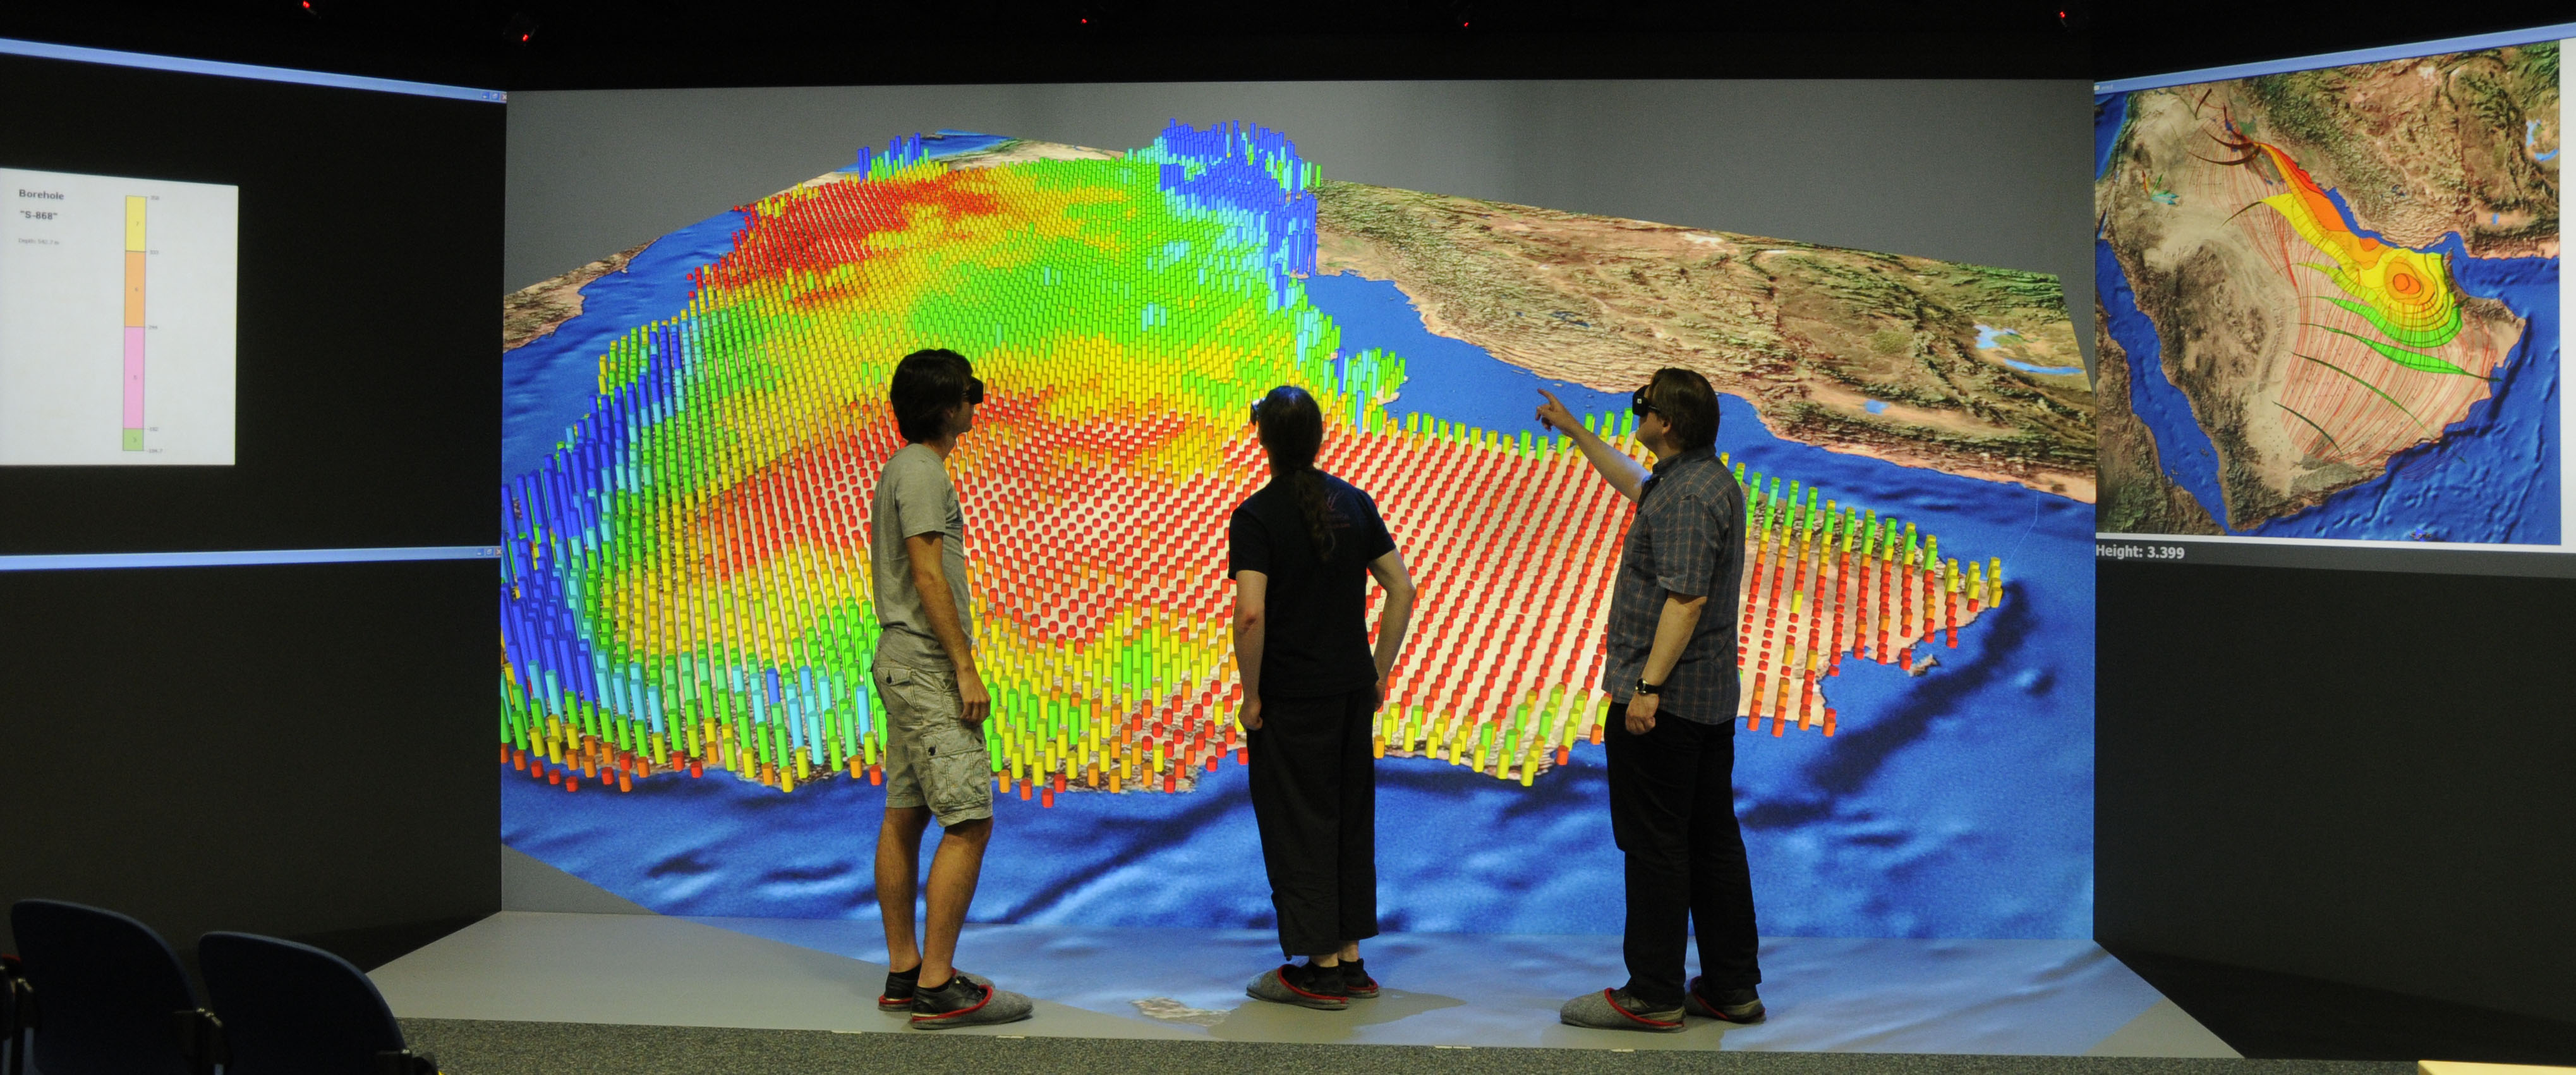
\includegraphics[width=1.0\textwidth]{images/sa_2d_3d.jpg}
\caption{Mixed 2D / 3D visualization of observed rain events on the Arabian Peninsula~\cite{rink:iwas}. In addition to the stereoscopic image on main screen, stratigraphies from interactively selectable borehole data (on the left) and an overview map (on the right), indicating the current observer position, are shown.}
\label{fig:sa}
\end{figure*}

\subsection{Mobile VR equipment}
\label{mobile-vr-equipment}

For off-site presentations such as on conferences, workshops or visits to project partners or stakeholders, we can also utilize mobile equipment to demonstrate the same visualization projects as in the \emph{VISLab} (although in a much smaller resolution and also limited to one concurrent user). The equipment consists of notebooks with dedicated GPUs and stereoscopic projectors or head-mounted displays such as the \emph{Oculus Rift}~\cite{web:rift} as shown in figure \ref{fig:rift}.

\begin{figure}[htb]
  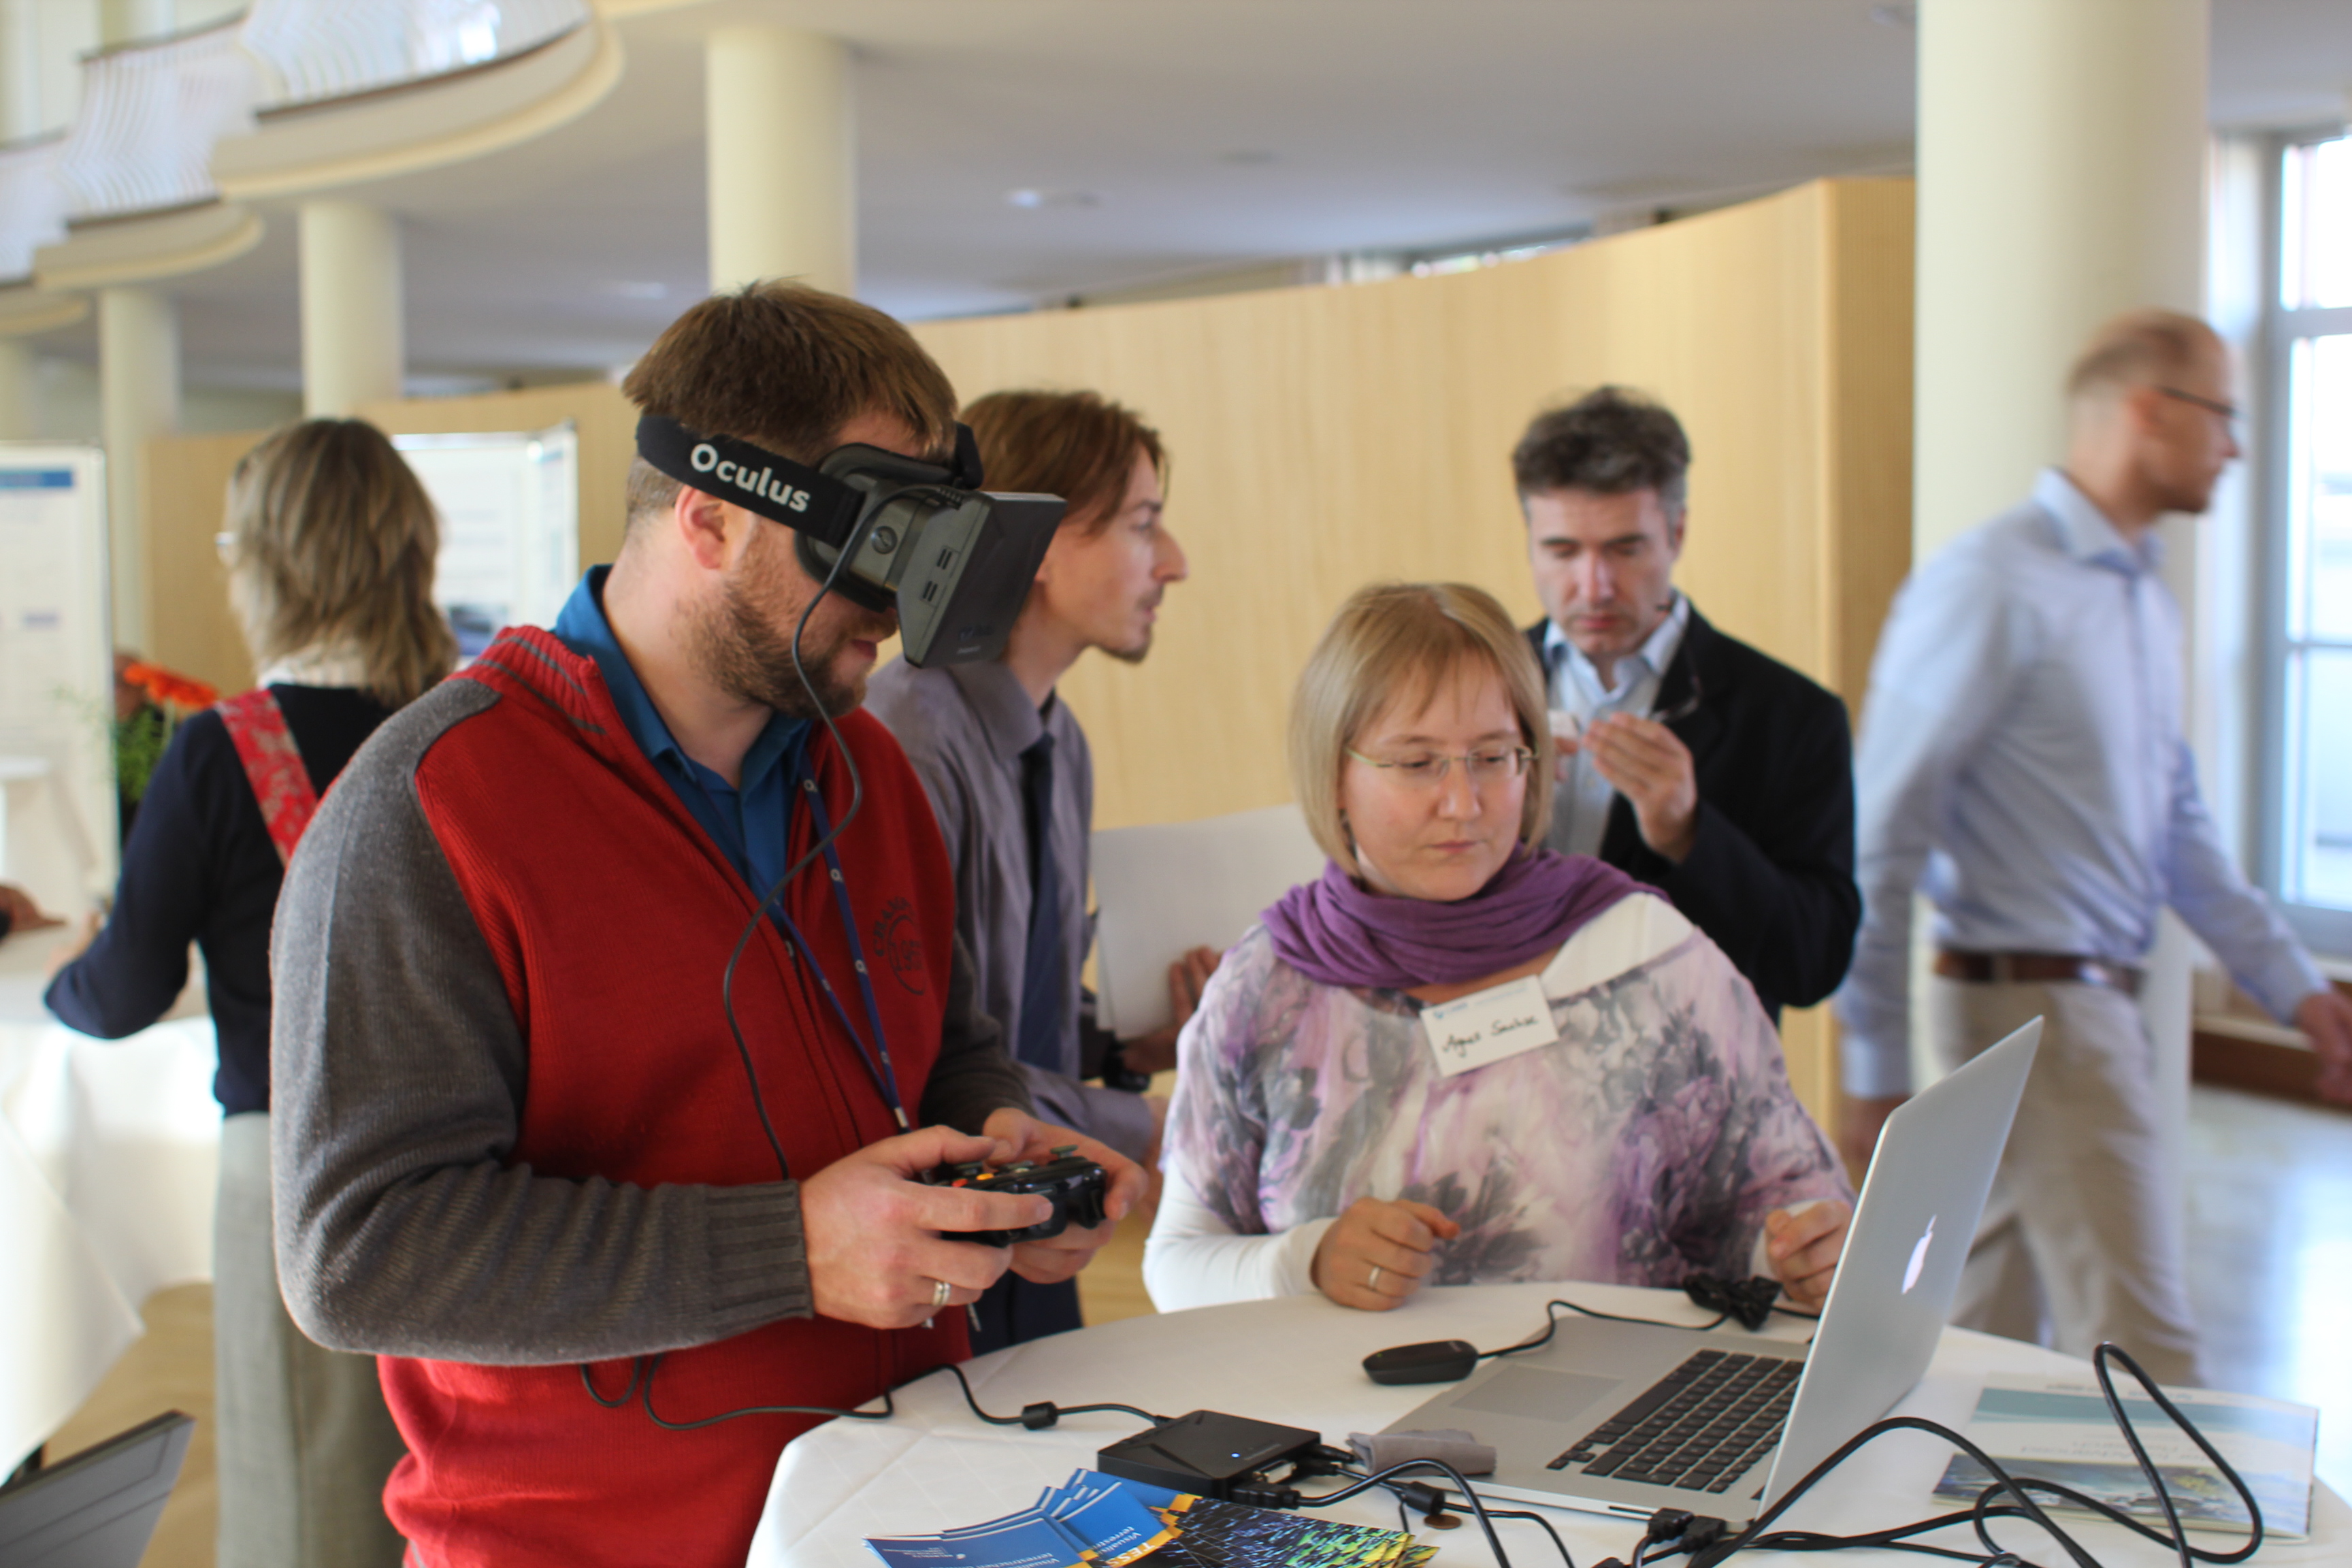
\includegraphics[width=\linewidth]{images/rift.jpg}
\caption{Mobile presentation with help of a head-mounted display and a game console like input controller at a scientific conference.}
\label{fig:rift}
\end{figure}

\subsection{Software}
\label{software}

Because of the clustered setup, we can only use software which can run in parallel and synchronizes the current state across all involved machines. There are specialized software with integrated cluster rendering capabilities and middleware software which add this functionality on top of non-clustered applications. These middlewares, such as \emph{Techviz}~\cite{web:techviz} or \emph{Conduit}~\cite{web:conduit}, intercept graphic commands from a desktop application and redistribute them to a render cluster. Such middleware software products allow to run a regular 3D desktop application in a VR environment with stereoscopy and tracking enabled. A data conversion is not necessary for this setup but interaction and presentation techniques are limited by the desktop application employed and performance is lost during graphic commands interception and distribution to the cluster such that immersion and feedback are severely affected.

Due to these disadvantages, we use software packages with native cluster rendering capabilities such as \emph{VRED}, \emph{ParaView} or \emph{Unity} in conjunction with \emph{MiddleVR}. All of these are introduced in the following:

\paragraph{VRED}
is a commercial software by \emph{Autodesk} (former \emph{PI-VR}) specialized in photorealistic real-time product rendering running on Windows~\cite{web:vred}. It is build on top of \emph{OpenSG}, an open-source scene graph library which offers clustered rendering~\cite{opensg}. \emph{VRED} can arrange imported 3D objects in a virtual scene, allows for tweaking of material (properties how the surface of the 3D objects reacts to lighting) and lighting parameters but is neither a modeling software nor are there many interaction possibilities besides viewer movement and object selection. It has a plug-in interface but no documentation is available from the vendor on how to address it. An advantage of the software is that \emph{VRED}'s editor can be directly connected to the \emph{VISLab}'s display so that local changes to the scene done at the presentation terminal are visible immediately on the video wall.

\paragraph{ParaView}
is an open-source data analysis and visualization software~\cite{paraview} by \emph{Kitware Inc.} build on top of the \emph{Visualization Toolkit}~\cite{vtk} (\emph{VTK}). Both technologies are also integrated in our visualization workflows (see \ref{workflows}). \emph{ParaView} allows to quickly create visualizations and implements a large number of well established visualization algorithms and techniques. It can run on distributed memory architectures to analyze large data sets and to drive VR displays. Using \emph{ParaView}, we can modify visualization parameters directly in the VR environment. Unfortunately, it lacks more sophisticated interaction and presentation features.

\paragraph{Unity}
is a complete game engine by \emph{Unity Technologies}~\cite{goldstone:unity3d}. It is available in a free and a commercial editor variant with the latter supporting more advanced rendering techniques (soft shadows, HDR, post-processing effects) and team collaboration features. \emph{Unity} has several rendering backends (\emph{OpenGL}, \emph{OpenGL ES}, \emph{Web\-GL}, \emph{DirectX}) so it can be run on all major platforms as well as on the Web (with an additional browser plug-in)~\cite{web:unity}. \emph{Unity}'s basic scope of operation does not include any interaction functionality but it has a comprehensive scripting documentation and a vivid plugin community so that it is very easy to integrate missing features. Application testing can be done directly in the \emph{Unity} editor by tweaking the application at runtime. However, \emph{Unity} created applications cannot run in a clustered environment. Therefore \emph{MiddleVR} is used.

\paragraph{MiddleVR}
is a generic virtual reality middleware from \emph{i'm in VR} designed to work with different 3D applications~\cite{web:middlevr}. It features a graphical configuration tool to setup VR systems independent of specific software. It implements interaction devices, stereoscopic rendering and clustering when using software not supporting this functionality. The \emph{MiddleVR} configuration is then used in a \emph{Unity} plugin to enable all these features in Unity applications. The \emph{MiddleVR}-enabled Unity application is VR system agnostic, once compiled it can be run on any VR system supported by \emph{MiddleVR}. A disadvantage of this approach is that the final application cannot be run inside the Unity editor but stand-alone, so that it cannot be altered interactively at runtime. The fact that a recompilation of the application takes just a few seconds weakens that drawback.

For the future, we will focus on the use of Unity as a platform for highly interactive visualizations to illustrate and discuss complex phenomena. In contrast, ParaView is more suited for rapid prototyping and exploration of complex data sets but will also play an important role in future workflows (see \ref{in-situ-visualization}).

\subsection{Workflows}
\label{workflows}

For simulation, we employ \emph{OpenGeoSys}~\cite{kolditz:ogs}, an open-source platform and flexible numerical framework for the simulation of thermo-hydro-mechanical / chemical processes in porous and fractured media with applications in geoscience and hydrology. In order to simulate these processes models are defined that include as much relevant data as possible to account for all phenomena defining that natural system. Heterogeneous data sets representing the model characteristics are given as input parameters to the simulation software which returns result data sets predicting system behavior in areas of interests.

We are both using visualization when setting up the model and simulation as well as to analyze simulation result data. As a basis for creating visualizations we employ \emph{VTK} which is also integrated into the \emph{OGS Data Explorer} framework (a data integration and visualization tool for pre- and postprocessing \emph{OpenGeoSys} simulation data~\cite{rink:eesenvirvis}) as well as \emph{ParaView}.

We provide utilities and \emph{ParaView} plugins to convert \emph{VTK} visualization data to formats supported by the VR frameworks used in the \emph{VISLab}, i.e.~OpenSG for \emph{VRED}~\cite{bilke:vtkosgconverter} and Autodesk FBX for \emph{Unity}~\cite{bilke:vtkfbxconverter}. Conversion can be either done manually in the \emph{OGS Data Explorer} or in a batch process by employing \emph{ParaView}'s Python scripting interface. The second approach is especially useful when converting large sequences of complex data sets such as time steps of simulation results from transient finite element models. During conversion, meta data is appended to the data sets to include information not necessarily supported in FBX such as a specific material and rendering setup or time stepping information. This meta data is evaluated when loading the data sets into Unity and can be queried, i.e.~for displaying the time stepping information as a text overlay. Multiple data sets can be arranged both in a spatial but also in a temporal context and a variety of presentation techniques (i.e. defining camera animations, fading in/out of data sets, selection of subsets, displaying additional information) are implemented, see~\cite{rink:eesenvirvis} for details.

\section{Overview of VISLab Applications}
\label{overview-of-VISLab-applications}

In the following, several case studies are presented which used our visualization workflows and utilized the \emph{VISLab}. Most of them have a background in hydrology, geosciences or energy but research projects furthermore include topics in urban planning and climate prediction.

\subsection{Ammer Catchment}
\label{ammer-catchment}

The catchment of the river Ammer in southwest Germany has been selected as the study region for a holistic analysis of the water cycle coupled to reactive solute transport, for addressing water and solute fluxes at the catchment scale as a function of and in feedback with changes in climate, land use, and water usage~\cite{grathwohl:wessti}. The river has a length of 25\,km and is a tributary to the Neckar. Its catchment has a size of 180\,km\textsuperscript{2} with a geology comprised of a sequence of Triassic strata forming a landscape characterized by escarpments~\cite{selle:wessti}. The Ammer is mainly fed by groundwater from the karstic and fractured aquifers and drains the catchment at a rate of ca. $1\,m^3/s$.

The finite-element groundwater model is based on a digital elevation model with a resolution of 100\,m in combination with interpolated subsurface layers based on the stratigraphic data of over 100 boreholes. For simulation purposes, the subsurface information has been combined into four separate layers, consisting of a part\-ly karstified limestone aquifer overlaid by Keuper-layers. In addition, the scene includes the stream network and groundwater production wells, which are employed as boundary conditions for the model as well as raster data with groundwater recharge information. Based on the results of a steady-state groundwater recharge simulation, the presentation also includes iso-surfaces representing the groundwater head as well as stream tracers for the visualization of flow paths within the catchment. See Selle et al~\cite{selle:wessti} for more information on the groundwater study and Rink et al~\cite{rink:wessti} for model setup and data visualization.

\subsection{Western Dead Sea - Sustainable Management of Water in Arid and Semi-Arid
Regions}
\label{western-dead-sea---sustainable-management-of-water-in-arid-and-semi-arid-regions}

The catchment of the Western Dead Sea (Israel / Palestine) was analyzed within the \emph{SUMAR}-Project and de\-mon\-strates a groundwater flow model of a semi-arid to arid case study which is coupled with a hydrological model. The climatic conditions exacerbate the tense situation of the drinking water supply for the 3800\,km\textsuperscript{2} large study area. And secondly, they lead to political and socio-environmental stresses. The overall aim of the \emph{SU\-MAR}-project~\cite{Siebert:2014} focuses on the quantity of surface and groundwater fluxes inside the catchment, which is influenced by faults of the Jordan Rift Valley System and were drained towards the shrinking, hypersaline and endoheric Dead Sea.

\begin{figure}[htb]
  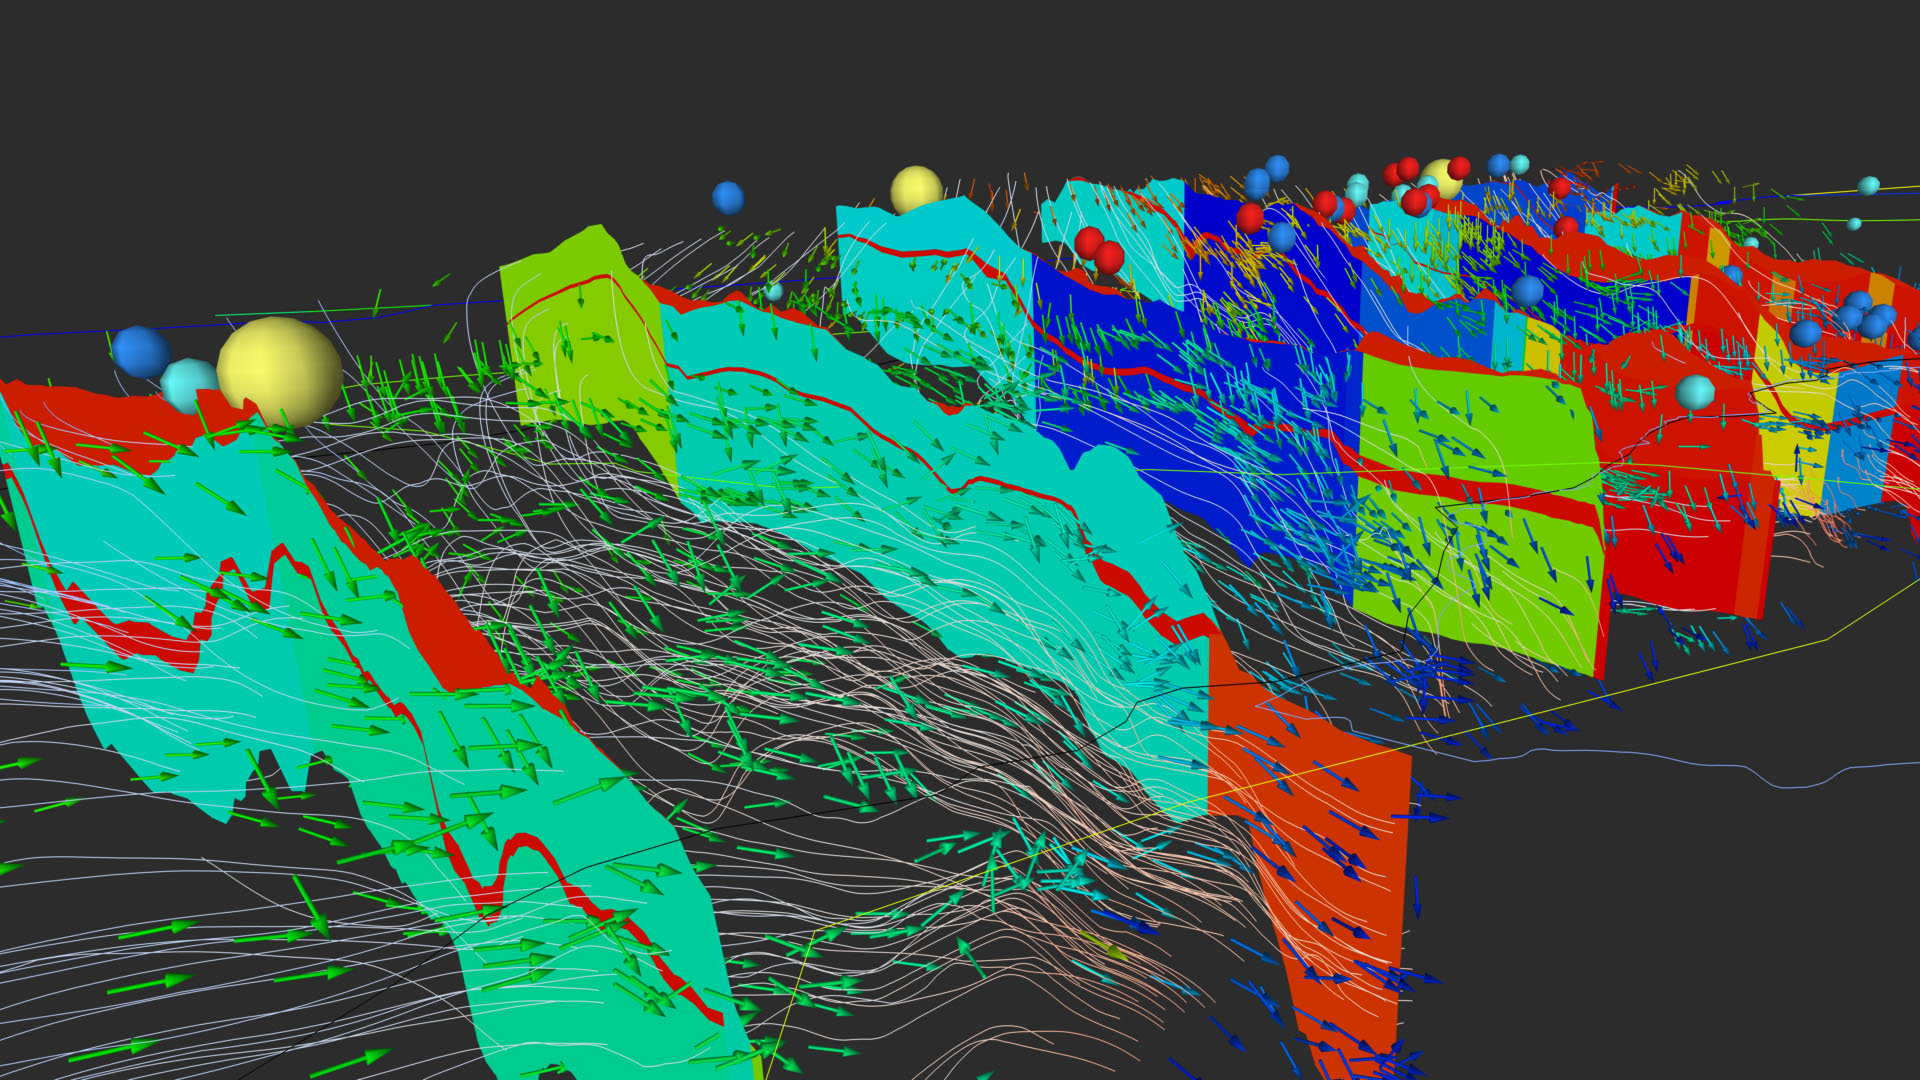
\includegraphics[width=\linewidth]{images/deadsea.jpg}
\caption{Cross section of the Upper and Lower Judea Group aquifer of the Western Dead Sea catchment, divided by an thin aquiclude (red line). The density of the groundwater flow paths with its velocity vectors describes the groundwater flow dynamics of the Cretaceous aquifer system from west of the catchment towards the Dead Sea. Colored spheres show the locations of wells, climate stations and cities for better orientation.}
\label{fig:deadsea}
\end{figure}

Several methods were applied to localize (with remote sensing data), to quantify (with 2D hydrological and 3D groundwater flow modeling) and to simulate water flow volumes and flow paths (with groundwater flow modeling~\cite{graebe:modelcare}) towards the Dead Sea. The study area is characterized by two Cretaceous limestone aquifers (confined / unconfined) of around 400\,m thickness including steep hydraulic gradients, which serve as the only fresh water resources in this region. Especially the visualization of the numerical groundwater flow model (see figure \ref{fig:deadsea}), which was implemented into OpenGeoSys, helps to detect uncertainties of the hydrogeological input data sets and enables a comprehension of the flow dynamics of the heterogeneous partly karstified limestone aquifer. To this end the calibrated steady state groundwater flow model provides quantifications of the water balance of the subsurface catchment and is the starting point for the transient modeling of surface and subsurface flow processes~\cite{graebe:wessti}. The hydrological model \emph{J2000g}~\cite{KrauseKralisch:2005, Krause:2001} was applied to estimate i.e.~the groundwater recharge of the widely distributed bare rock soil cover for a 30 years period. Its result was transferred as a time dependent boundary condition to the 3D finite element mesh nodes with a resolution of 250\,m and represents by its trend the continuous lowering of the water level in the aquifer system due to over pumping issues.

\subsection{Nankou - Groundwater deterioration in a suburban area of Beijing}
\label{nankou}

Nitrate contamination of groundwater resources is a severe environmental problem worldwide, mostly caused by extensive agriculture using large amounts of fertilizer to increase plant productivity. Nitrate has extreme long residence times in the subsurface and remediation is therefore hampered and requires costly long-term efforts. Therefore, simulation and visualization are important tools for planning and optimization of remediation scenarios. Figure \ref{fig:nankou} depicts the visualization of an OpenGeoSys subsurface model for the development of remediation setups of nitrate contaminations in China (\emph{Nankou} project) using the VR environment of the \emph{VISLab}. To present complex hydro-geological structures and results of nitrate remediation in the Nankou area to stakeholders and decision-makers of the Beijing district, 3D visualization techniques have been successfully used to foster both understanding and discussion of the invoked environmental problems within the geographical context, data availability and simulation results for the Nankou nitrate remediation project in China~\cite{sun:ees}.

\begin{figure}[htb]
  \includegraphics[width=\linewidth]{images/nankou.jpg}
\caption{A simulated ground water flow system is shown around pumping wells in the Nankou area with nitrate concentrations as colors on the streamlines.}
\label{fig:nankou}
\end{figure}

\subsection{Oman - Saltwater Intrusion Modeling}
\label{oman---saltwater-intrusion}

Within the project \emph{International Water Research Alliance Saxony} (IWAS), one of the main goals was to assess and evaluate water resources under various natural and human induced stress conditions. Several subprojects considered study regions in different parts of the world~\cite{kalbus:ees}.

\begin{figure}[htb]
  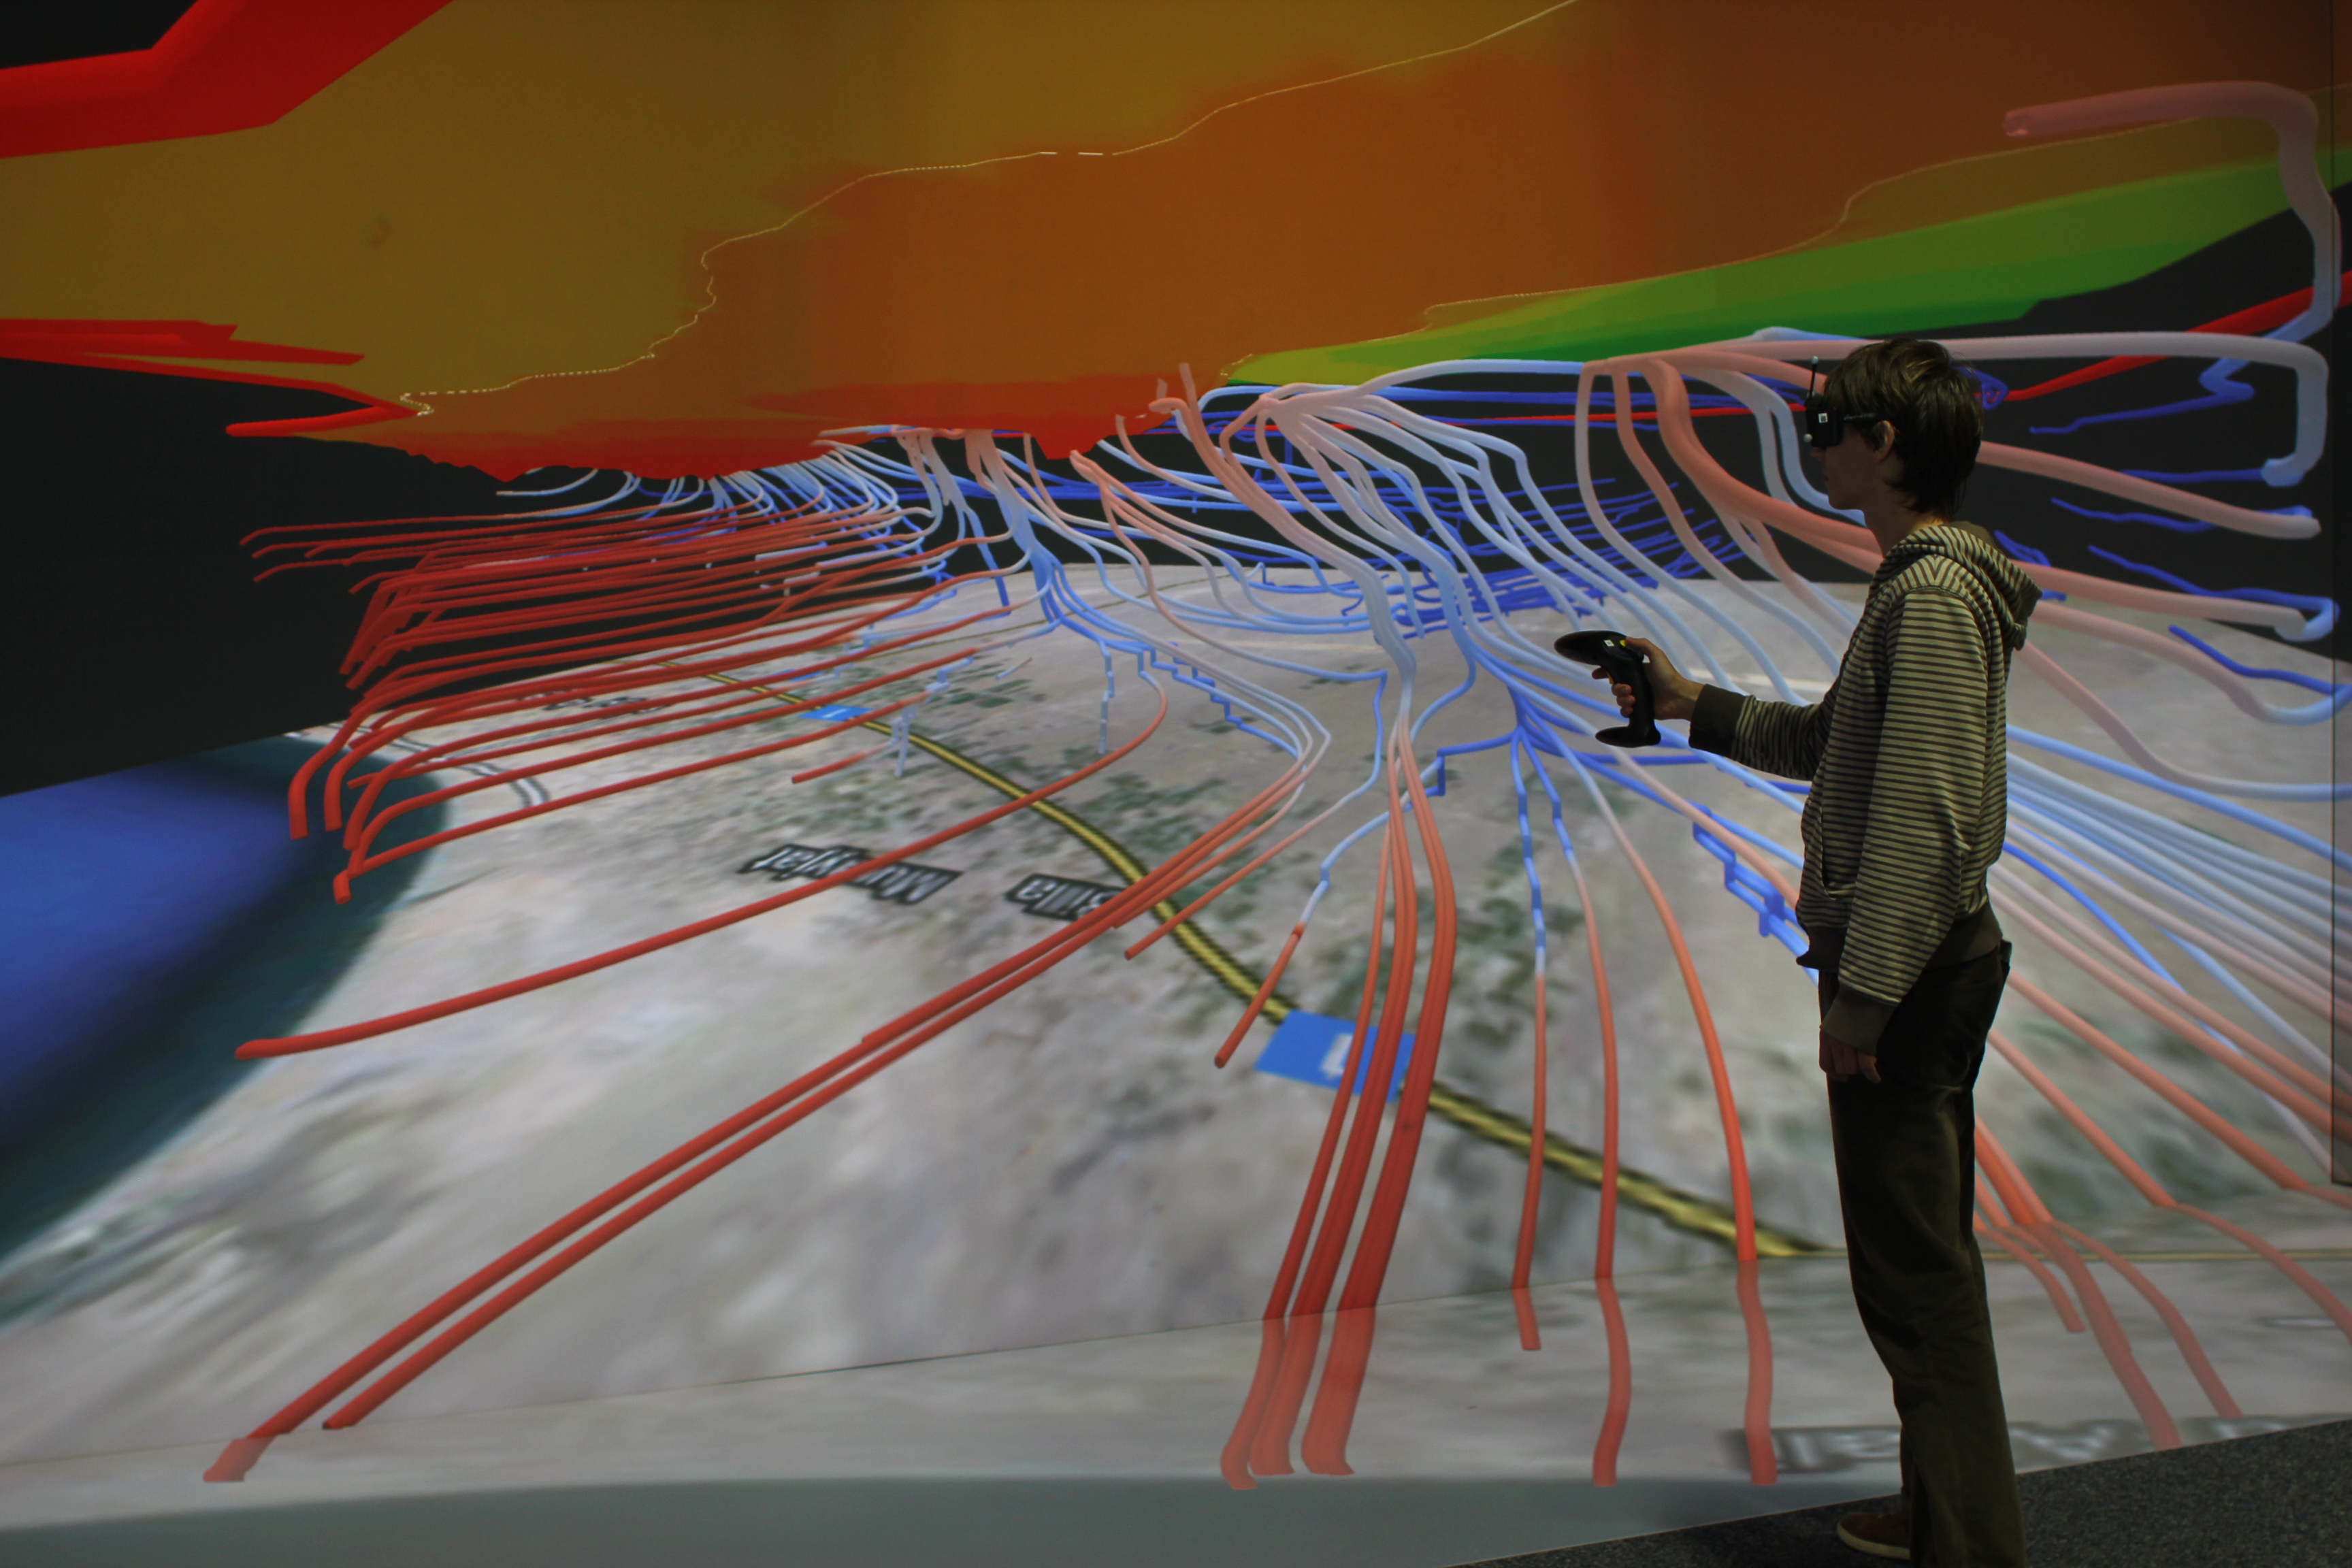
\includegraphics[width=\linewidth]{images/oman.jpg}
\caption{Analyzing groundwater flow patterns at the near coastal salt/freshwater interface (red/blue color on streamlines) in combination with groundwater surface drawdown due to pumping activities for determining subsurface water vulnerabilities utilizing the stereoscopic mode of the VISLab.}
\label{fig:oman}
\end{figure}

One of these case studies, a region scale study on density driven flow in a coastal aquifer that is used as source for agriculture irrigation, intensively made use of visualization options during model setup, verification of the variable density process, and for the transfer of knowledge to local authorities~\cite{walther:cam, walther:eesenvirvis}. Firstly, visualization was used to investigate plausibility of the set up hydro-geological model, that was constructed based on an extended inverse weighting distance interpolation~\cite{walther:modelcare}. Secondly, large data sets of model calibration and long term scenario simulations of the saltwater intrusion process were analyzed by utilizing \emph{ParaView}. \emph{ParaView} was run on a parallel cluster computer to omit bandwidth limitations to copy large data and to reduce computational burden on standard desktop machines. Thirdly, results of the modeling were visualized, which helped during discussions with experts and tremendously aided in knowledge transfer during a visit of Omani authorities from the Ministry of Regional Municipalities and Water Resources. Additionally, throughout all states of model development, calibration, scenario analysis, and result presentation, the \emph{VISLab} was utilized~\cite{walther:eesenvirvis}.

\subsection{TERENO-Observatory Harz/Central German Lowlands}\label{tereno-bode}

TERENO is a large-scale project aims to catalogue the longterm ecological, social and economic impact of global change at regional level~\cite{zacharias:tereno}. Four areas in Germany have been selected and are now heavily instrumented to allow extensive studies and simulations for researchers from different disciplines. Hydrogeological analysis in central Germany is being conducted in the catchment of the River Bode with a size of 3,100\,km\textsuperscript{2}. Within that area a number of intensive test sites have been selected, ranging in size from a small area of about one hectare, concerned with assessment of water balance in a forested region, to the complete catchment of one of the Bode's tributaries with a size of over 450\,km\textsuperscript{2} where hydrological processes in the stream as well as in the hyporheic zone are investigated~\cite{schmidt:selke, trauth:flow} as shown in figure \ref{fig:streambed}.

\begin{figure}[htb]
  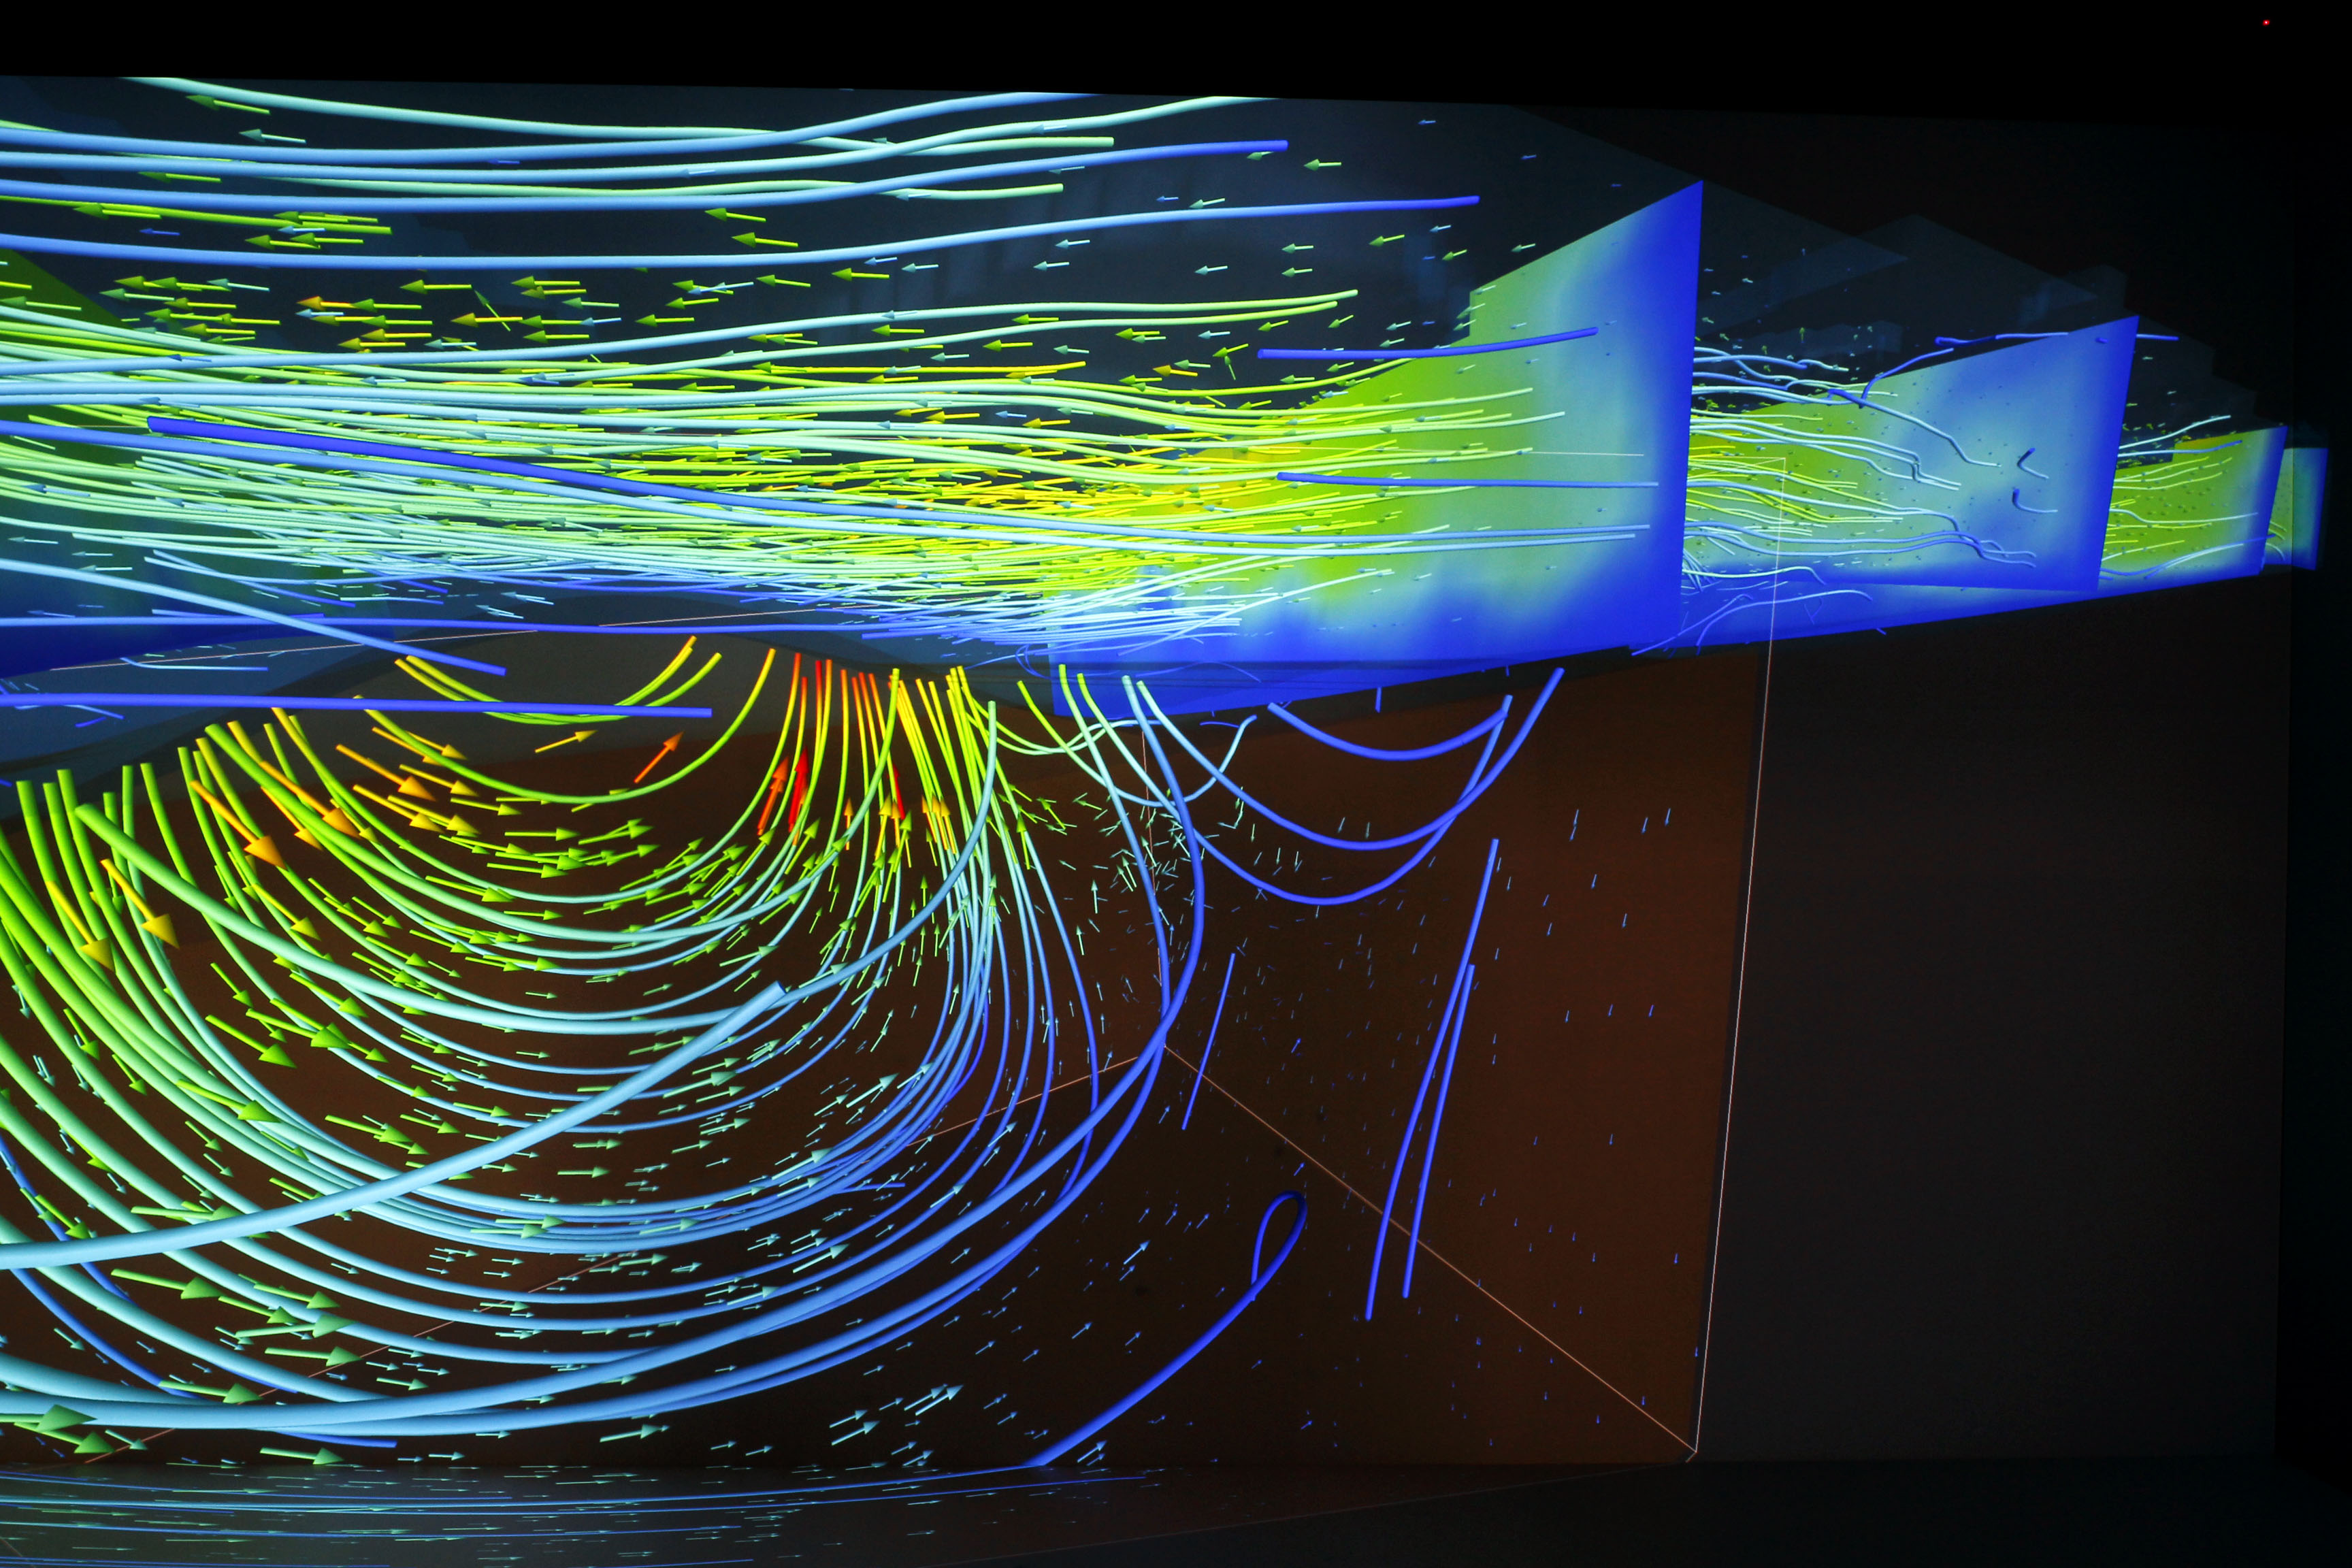
\includegraphics[width=\linewidth]{images/streambed.jpg}
\caption{Liquid flow turbulences in a streambed (top) are concurrently visualized with water intrusion in the underground forming a ground water flow system (bottom).}
\label{fig:streambed}
\end{figure}

The presentation consists of over $70$ heterogeneous data sets of different scale and resolution. Most notable are surface representations, consisting of a terrain model of the whole region with over 1 mio triangles with a max edge length of 30\,m. Terrain models of the intensive test sites also exist at a much finer resolution, ranging from 30\,m for the larger regions to just 1\,m for the regions covering 1\,km\textsuperscript{2} or less. Various color transfer functions or textures can be applied to these surfaces, including elevation information, soil moisture, or indication of land use. While textures are originating from raster data, transfer functions are based on statistical data or look-up tables. Geometrical information includes the courses of streams at various resolutions and displayed with different prominence. Furthermore, the scene includes climate stations, measurement networks, bathymetries of some of the larger water bodies within the region, structural models for the subsurface of two intensive test sites, borehole data and much more. Most regional data sets are only visible when the presentation zooms in on the intensive test site they are located in, to avoid unnecessary clutter of the overall scene. Still, data integration of so many data sets acquired by different means is quite challenging. A number of different preprocessing steps were required for concurrent display and visibility of small data sets within the larger context~\cite{rink:wessti, rink:eesenvirvis}.

\begin{comment} % TODO

\subsection{Gro{\ss}-Sch\"onebeck - Geothermal Energy}
\label{grouss-schoenebeck---geothermal-energy}

Norihiro Watanabe

In geosciences we have to deal with complex geological structures containing different architectural elements such as layers, faults, diapirs, fracture networks. Thermo-hydro-mechanical-chemical processes under extreme thermodynamic conditions have to be considered for utilizing geological reservoirs, i.e.~for geothermal energy~\cite{zehner:uncertainty}

\end{comment}

\subsection{PROTECT - Prediction of deformation to ensure carbon traps}
\label{otway-basin---co2-storage}

The \emph{PROTECT} project~\cite{krawczyk:deformation} is a partner project of the Australian \emph{CO2CRC Otway} project~\cite{cook:carbon}. Its aim is to determine the seismic and sub-seismic characteristics of potential fluid migration pathways between reservoir and surface. The goal of this part of the \emph{PROTECT} project that is presented here, was to generate an interactive visualization that combines original geophysical (i.e. seismic data and borehole data) and derived data (i.e.~seismic attributes like coherency), a geological 3D model~\cite{ziesch:geology}, as well as modeling results (from kinematic retro-deformation and geomechanical forward modeling) into an immersive presentation which can be shown on VR display systems.

The first steps were the visualization of our high-resolution, geological 3D model and the 3D seismic data set in ParaView. Conventional 3D P-wave seismic data can image faults with an offset of hundreds of meters down to circa 20 meters. Using seismic attributes (i.e. variance) and visualization of the results within an VR environment, we were able to identify faults with smaller offsets (between 10 and 20 meters). This complements the detailed 3D seismic interpretation and thus helps to identify possible pathways for injected $CO_{2}$.

3D seismics in SEG-Y format cannot be directly imported into \emph{ParaView}, so that a data conversion tool for seismic data was developed~\cite{bilke:simpleseismicreader}. It imports rectilinear-shaped seismic data in a plain text format into \emph{ParaView} using \emph{OpendTect}~\cite{web:opendtect}.

\begin{figure}[htb]
  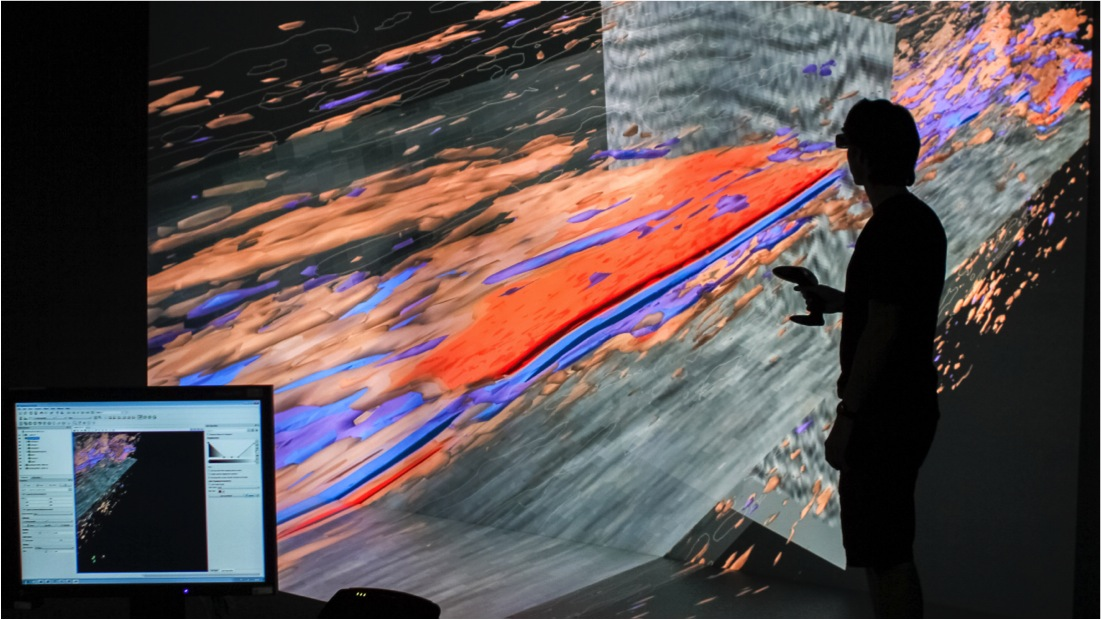
\includegraphics[width=\linewidth]{images/seismic.jpg}
\caption{ParaView running in the VISLab showing a spatial subset and cross-sections of 3D seismic data and isosurfaces of interesting features.}
\label{fig:seismic}
\end{figure}

\begin{comment} % TODO

\subsection{Thuringian Syncline - Faults modeling}
\label{thuringian-syncline---faults}

The \emph{INFLUINS} project investigates the movement of fluids in the subsurface in the Thuringian Syncline which covers most of the federal state Thuringia in Germany. Due to the formation history, the syncline contains many fault zones. The focus of the project is on the flow from the region of the uppermost soil layer down to the basement at depths in several kilometers including the effects of fault zones. In the \emph{INFLUINS} project the visualization is used to get a better understanding of the course of the stratigraphic layers, the integration of faults zones in the subsurface model and to examine the quality of the mesh elements. (TODO Ausführlicher) Furthermore the visualization is a valuable tool to interpret the simulation results.

TODO Bild kommt, wenn das erste sinnvolle Modell gerechnet ist.

\end{comment}

\subsection{Climate Data}
\label{climate-data}

In this case study, simulation data of the \emph{Weather Research and Forecasting} (WRF) model are visualized in combination with observation data from weather stations (i.e.~amount of precipitation at a station) and time independent static data (i.e.~river networks, cities) to analyze it and detect correlations and inconsistencies. The case study area is situated in northern central Europe with an expansion of about 1,300 by 580\,km. It includes various landscapes such as the Alps, lowlands of France, and the English Channel. This area is a common domain for regional weather simulations as it is an area of propagation of frontal systems. The case shows a winter situation on the 28th of January 2012 where the air was moist and cold.

For a detailed analysis of processes such as convection and heat transport, subsets of the area are defined. Figure \ref{fig:wind} shows an example of such a subset, where we concurrently visualized wind fields, mass fraction, humidity and heat fluxes in relation to the digital elevation model. The visualization is used to provide a detailed look at processes and investigate if they have been captured correctly by the model. Different time steps are displayed in an animated manner and the user can i.e.~analyze the development of convection, observe heat transports or study wind fields. The challenge in analyzing these data sets is their highly multivariate character that requires stereoscopic 3D visualization for analysis. The visual combination of simulation, observation, and statical data, which differ in their spatial and temporal resolution, supports the scientists to verify, falsify and generate their hypothesis~\cite{helbig:eesenvirvis}.

\begin{figure}[htb]
  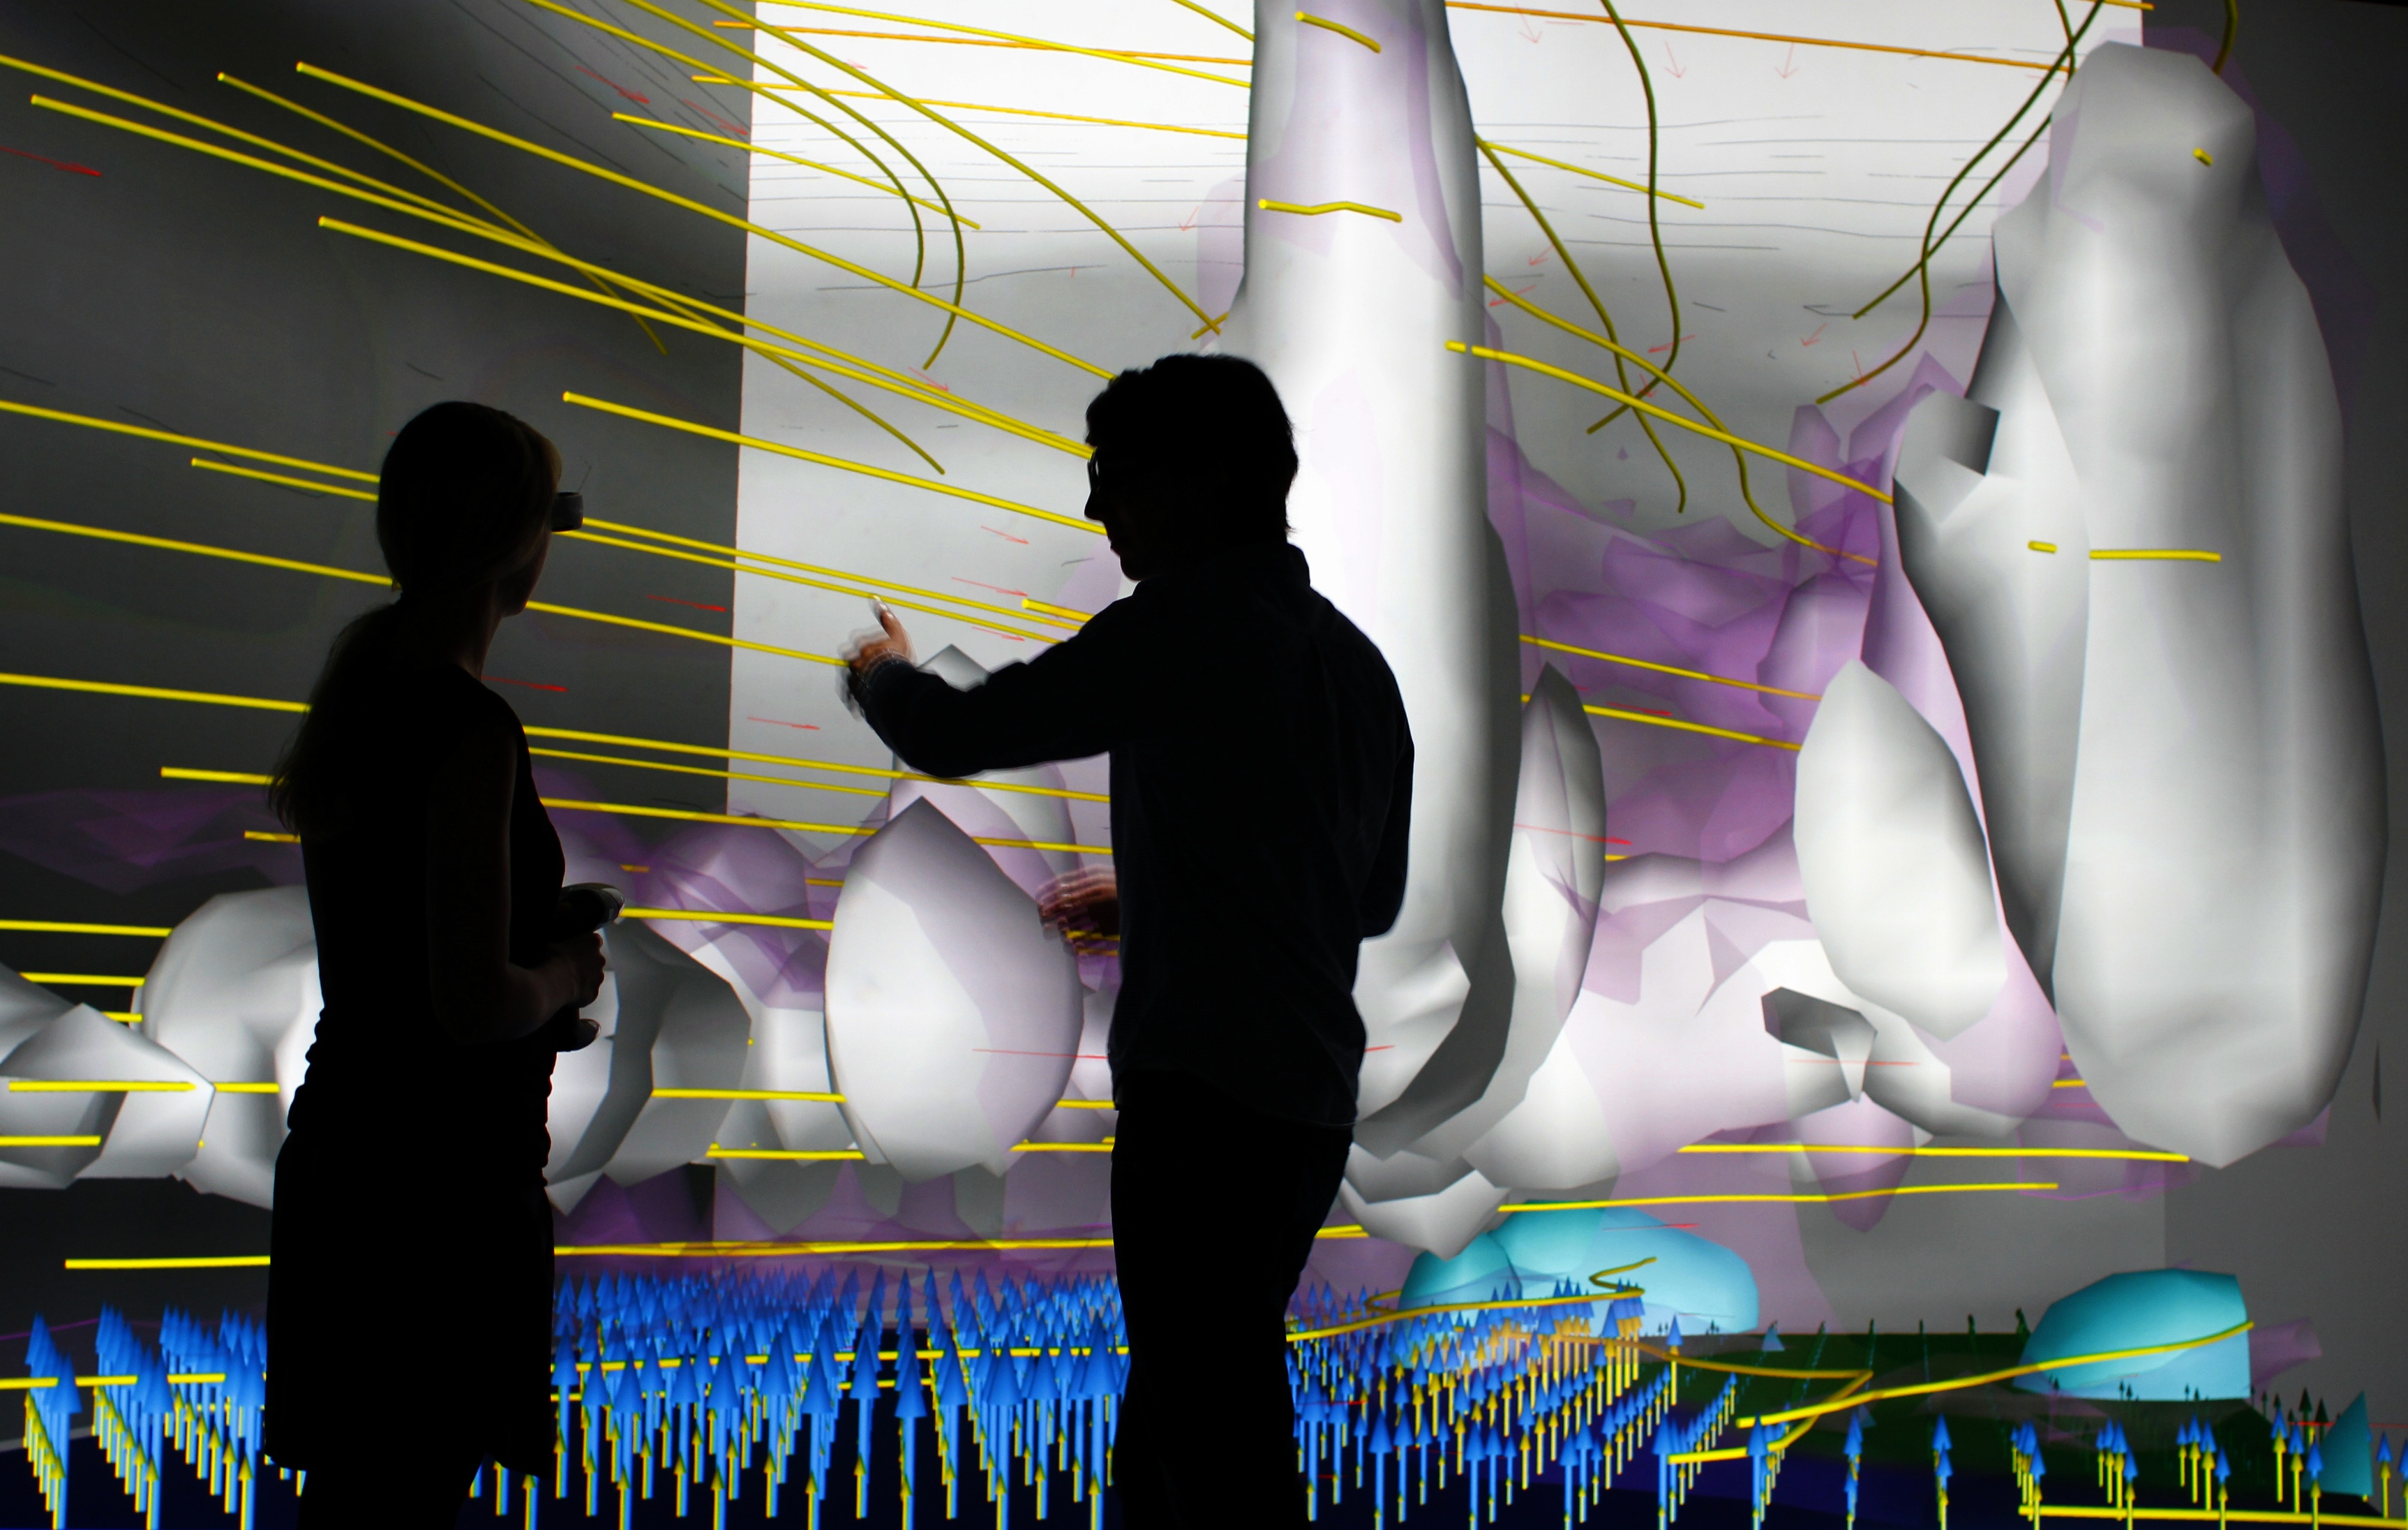
\includegraphics[width=\linewidth]{images/wind.jpg}
  \caption{Climate simulation data visualization showing wind fields (streamlines), mass fraction (white and blue isosurfaces), humidity (slices in the back) and heat fluxes (arrow glyphs on the surface) above the digital elevation model.}
\label{fig:wind}
\end{figure}



\subsection{Pore-Scale}
\label{pore-scale}

For a~detailed understanding of fluid flow behaiviour on the~pore-scale in
unconsolidated sediments simulations of the~incompressible Navier-Stokes
Equations were performed.
The unconsolidated artificial (\emph{in-silico}) sediments were generated with
the~SettleDyn software~\cite{web:SettleDyn} and prepared as input meshes for
a~finite volume method;
The~OpenFOAM simulation software~\cite{web:OpenFOAM} was used to obtain
a~solution of the~incompressible Navier-Stokes Equations in the~pore network
geometry.
Additionally a~particle tracking method was applied to simulate particle
deposition on the~grains' surfaces.

For the~particular realization of the~randomly generated porous medium we
studied the~fluid flow patterns in the~pores and distribution of
the~sticking particles on the~surfaces of the~grains.
Especially the~local fluid-flow structures were of interest.

For the~visualization of multiple domain boundaries we used a~two-sided material
rendering technique (described in detail in~\cite{naumov:twosidedrendering})
obtaining an~unobscured view on the~local fluid flow visualization
simultaneously keeping the~reference to the~geometry.
The~following Figure~\ref{fig:porescale} depicts particle visualization with
two-sided materials rendering.


\begin{figure}[htb]
  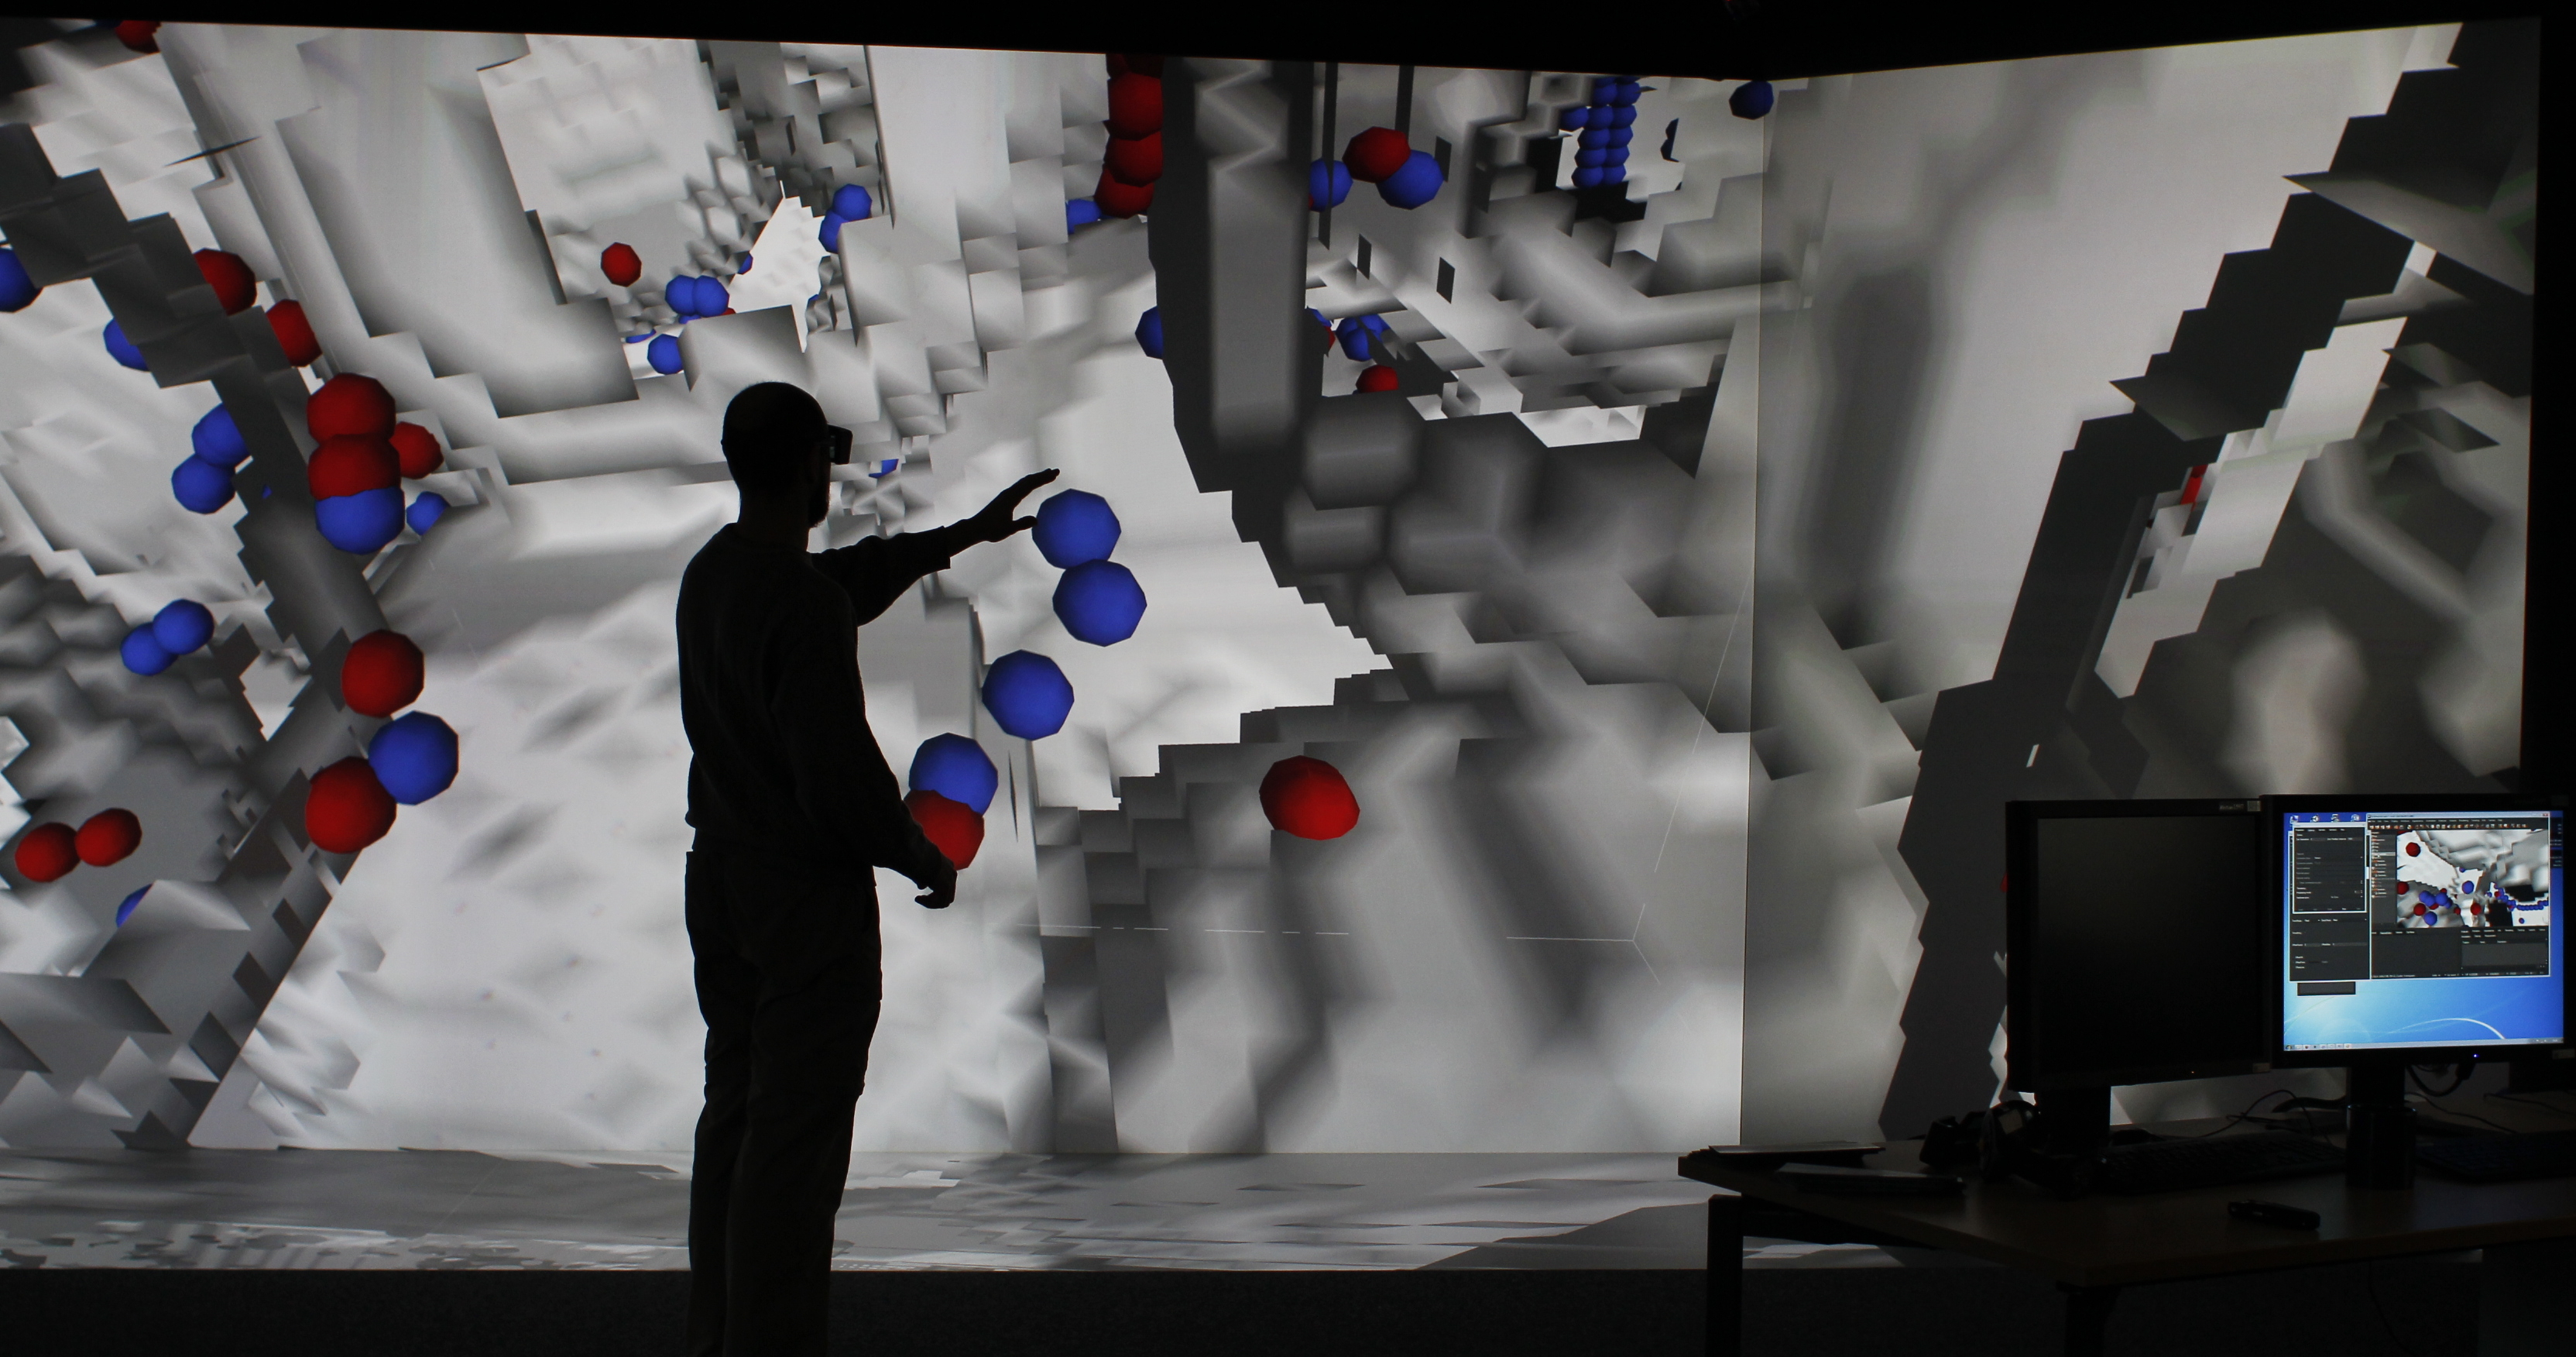
\includegraphics[width=\linewidth]{images/porescale_vislab.jpg}
  \caption{Pore-scale visualization of sticky particles on grains' surfaces.
  The~actor is looking from inside of a~grain looking through it; The~others
  grain's surfaces shown from outside are rendered opaque.}
\label{fig:porescale}
\end{figure}


\begin{comment} % TODO
\subsection{Biodiversity in Rain Forests}
\label{biodiversity-in-rain-forests}

Andreas Huth Formind \cite{kohler:98}

\begin{figure}[htb]
  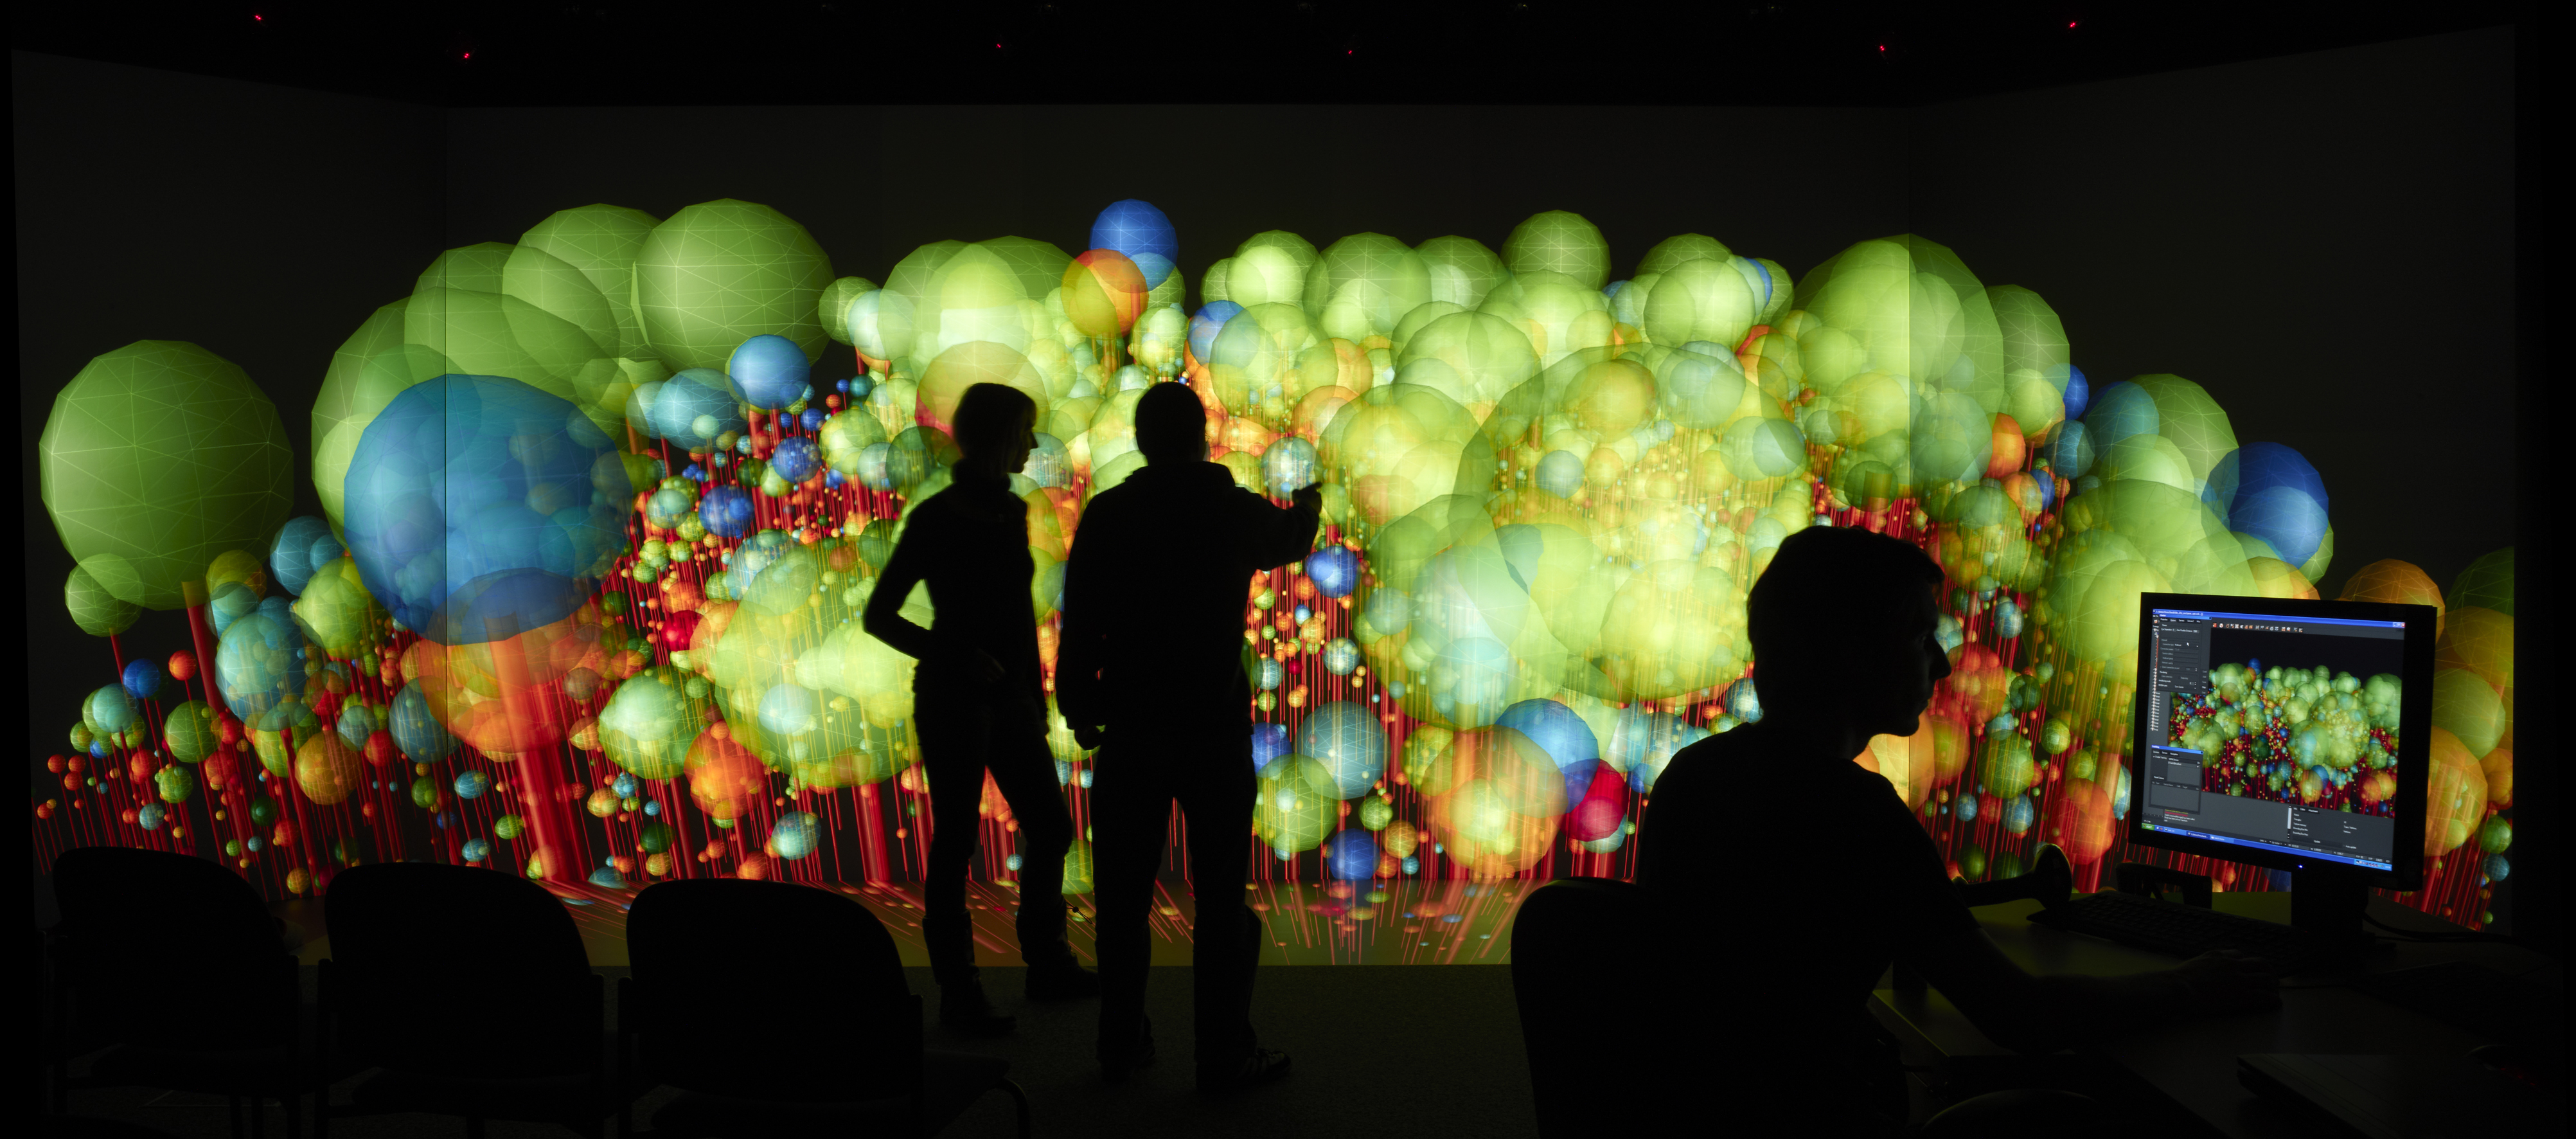
\includegraphics[width=\linewidth]{images/biodiversity.jpg}
\caption{TODO}
\label{fig:biodiversity}
\end{figure}

\subsection{Windpark Planning}
\label{windpark-planning}

Bj\"orn Zehner \cite{zehner:windpark}

\end{comment}

\subsection{Urban Environments}
\label{urban-environments}

% TODO put on GitHub and DOI

To help in the creation of urban environment visualizations usable for social sciences and for urban development a procedural\cite{procedural:modelling} building model generator was developed~\cite{bilke:master}. The software called \emph{CityGenerator} allows to procedurally generate building models as well as small city scenes as shown in figure \ref{fig:city} out of simple building blocks such as fa\c{c}ade textures, doors, windows and decoration elements. The user can specify input parameters including the building footprint, building height and designs a template fa\c{c}ade in a graphical user interface. This template fa\c{c}ade is defined by a set of grammatic rules~\cite{procedural:buildings}. The actual model generation is implemented as a \emph{VRED}-plugin allowing for immediate presentation in the \emph{VISLab}. \emph{Level-of-detail} (LOD) techniques ensure a good performance of larger scenes.

\begin{figure}[htb]
  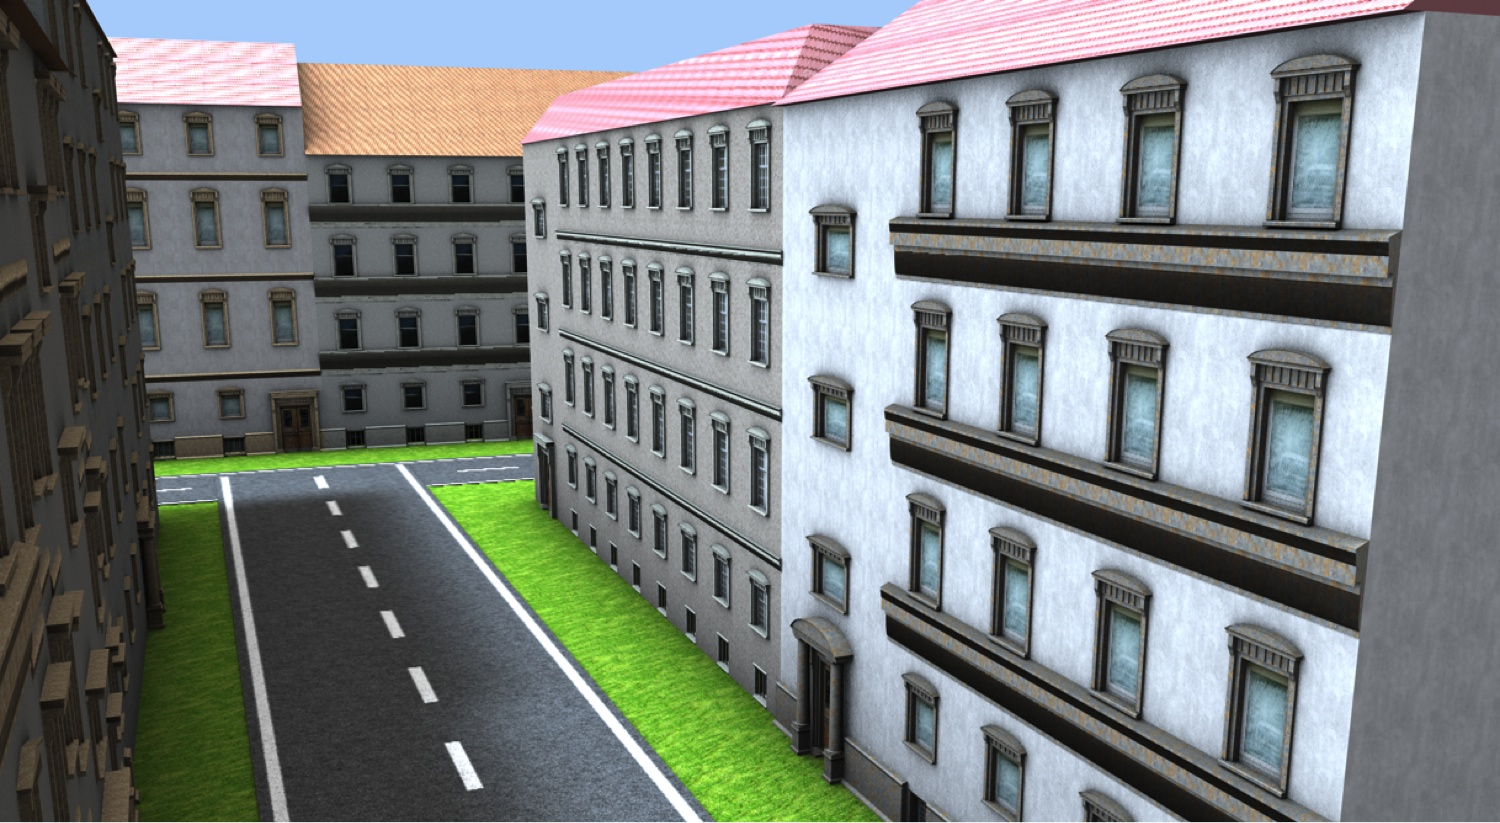
\includegraphics[width=\linewidth]{images/city.jpg}
\caption{Facades and building models in the style of the historic period of promoterism were used as examples to demonstrate the ability of the procedural city generation system.}
\label{fig:city}
\end{figure}

\section{Future work}
\label{future-work}

For the future, we would like to foster the usage of scientific visualization in the daily research work. All software and tools we develop are freely available and open source. Accessibility to these tools is crucial so we are aiming to provide a comprehensive documentation~\cite{web:ogs-docs} which can be enhanced with video tutorials in the future and we also arrange training courses several times a year and organize workshops at visualization conferences~\cite{web:envirvis}.

To face the challenge to visualize increasingly complex models and simulations, especially in the field of high-performance computing (HPC), we will integrate visualization methods into simulation codes. A simplification of the technical setup of the \emph{TESSIN VISLab} will unlock more fields of applications.

\subsection{In-situ visualization}
\label{in-situ-visualization}

\emph{In-situ}- or \emph{Co}-visualization allows to create result analysis and visualization as a part of the simulation process. By observing the simulation process it is possible to detect errors in the input data early. The user can then cancel the simulation, adapt the input data and restart the simulation. This saves computing time, decreases the workload of scientists and give rise to an effective iterative process of refining and adapting the simulation. Because the \emph{in-situ} visualization can be run without user interaction, it can also be useful for software quality management and benchmarking by automatically comparing visualization output and analyzed data between different program versions.

Normally, the simulation process is divided into four parts: during \emph{preprocessing} the raw input data is transformed and validated. The \emph{model setup} configures the involved model for the given problem appropriately. Typically the \emph{simulation} step produces large amounts of result data, especially in the field of coupled process simulations, which are then processed and analyzed in the \emph{postprocessing} step to reduce data by significance and to identify interesting aspects. Usually the postprocessing takes place on frontend-nodes of the HPC system or on the users machine where storage capacity may be limited. In the latter case all result data have to be transfered over the computer network which can be the limiting factor in various applications. The analyzed data as the outcome of the postprocessing step can be much smaller than the simulation result data.

Therefore, the postprocessing should become integrated into the simulation itself to avoid the communication bottleneck by transferring the analyzed data only and to allow users to monitor their simulated processes to ensure reasonable behavior.

We started using the library \emph{Catalyst}~\cite{web:catalyst} for integration of such an \emph{in-situ} visualization system into \emph{OpenGeoSys}. \emph{Catalyst} is an extension of \emph{VTK} / \emph{ParaView}. On the basis of a representative example data set the user defines a visualization pipeline (either by a script or interactively in \emph{ParaView}) which is then executed after defined time step intervals of the simulation. During simulation time the user gets processed data as a result of the visualization pipeline, images of the visualization and an interactive remote visualization in \emph{ParaView}.

Furthermore, it should be possible to view the remote visualization in the VR environment of the \emph{VISLab}, which is also connected to the HPC system of the UFZ via a fast computer network (\emph{Infiniband}).

\subsection{Simplified hardware setup}
\label{simplified-hardware-setup}

Our current hardware setup limits the usable 3D applications to software which can be run in parallel and synchronized on a computer cluster. This rules out the usage of commonly used software in environmental sciences such as geographic information systems (GIS). Novel high resolution projectors can help us to reduce the number of projectors for our display from 13 to 8 in which the main screen is driven by one 4K (Ultra HD resolution) projector instead of six SXGA projectors while also increasing the pixel count by approximately 30 \%. This allows the usage of every 3D enabled application when disclaiming the projection on the floor and side screens. Also startup times of the display will be much faster and overall system reliability is improved. The technical implementation of such a setup in combination with the remaining projectors on the floor and side screens is currently under review. An additional wireless presentation system~\cite{web:clickshare} entitles even people not familiar with the display system a straightforward usage of it.

%\bigskip
% \myedit{}{Du solltest vermutlich noch ein Acknowledgement einf\"ugen, in dem du auf die Danksagungen in den jeweiligen Papern verweisst. Damit sich niemand vergessen f\"uhlt\dots}

%%%%%%%%%%%%%
%% ENDCONTENT
%%%%%%%%%%%%%


\begin{acknowledgements}
The authors would like to thank Benny Selle, Nico Trauth, Thomas Kalbacher and Feng Sun for providing some of the data sets presented in the case studies. Further acknowledgements to particular project funding are referred to in the individual papers cited for the case studies presented in this article.
\end{acknowledgements}

% BibTeX users please use one of
%\bibliographystyle{spbasic}      % basic style, author-year citations
\bibliographystyle{spmpsci}       % mathematics and physical sciences
%\bibliographystyle{spphys}       % APS-like style for physics
\bibliography{vislab}   % name your BibTeX data base

\end{document}
% end of file template.tex

